\chapter{Misión de vuelo}   

En esta sección se describe el proceso de implementación de los comandos de vuelo y el algoritmo de seguimiento de trayectoria para el vuelo a través del circuito; cabe mencionar que se siguió un paradigma similar al de la sección anterior, primero se trabajó con scripts individuales de Python, y una vez que se validó su funcionamiento, se creó su respectivo nodo en ROS; los resultados correspondientes a este último punto, se tratan a detalle en el capítulo dedicado a ROS.

Dicho lo anterior, el algoritmo de seguimiento de trayectoria se trabajó en pequeñas etapas, en donde se probaba una funcionalidad distinta del piloto automático, de tal forma que cada etapa integra a la anterior, y así de forma sucesiva hasta que se obtuvo el script con el algoritmo de misión de vuelo. Los códigos fuente pertenecientes a cada etapa se encuentran en el respectivo repositorio de GitHub, perteneciente al presente trabajo. La tabla \ref{tab:pymavlink} muestra la relación que existe entre cada etapa y su script en el repositorio de GitHub.

\begin{table}[ht]
    \centering
    \begin{tabular}{lll}
        \hline
         No. & Etapa & Código fuente\\
        \hline
        \hline
        1 & Establecimiento de la conexión entre Pymavlink y ArduPilot & listen.py\\
        2 & Configuración del modo de vuelo del dron & mode.py\\
        3 & Armado de motores y despegue & takeoff.py\\
        4 & Seguimiento de trayectoria con waypoints & movement.py\\
        5 & Implementación de la misión de vuelo & mission.py\\
        \hline
        \hline
    \end{tabular}
    \caption{Relación entre etapa y su código fuente}
    \label{tab:pymavlink}
\end{table}

A continuación se muestran los resultados obtenidos en cada una de las etapas mencionadas. 

\section{Conexión entre Pymavlink y ArduPilot}

Inevitablemente, lo primero que se realizó fue comprobar la comunicación entre el script de Pymavlink y el SITL de ArduPilot. Por esta razón, el script perteneciente a esta etapa es bastante sencillo; sin embargo, representa la base de las subsecciones posteriores.

A grandes rasgos, lo más destacable es la inclusión de la librería Pymavlink y la creación de un objeto que sirve como intermediario entre el script y el piloto automático simulado. Dicho esto, para crear el objeto es necesario especificar la dirección que se utilizará para entablar la conexión; esta se especifica al momento de iniciar el SITL de ArduPilot en un terminal. Además, ArduPilot provee dos direcciones para realizar la conexión. En este caso, se escogió la \textit{14551} de forma arbitraria, sin ninguna razón en específico. La figura \ref{fig:Ardupilot_Py} muestra la información generada por ArduPilot durante el inicio de una instancia del SITL, a simple vista es mucha información; sin embargo, los datos de interés para esta subsección se encuentran en la línea en donde se indican las direcciones disponibles para recibir los datos manejados por el piloto automático, al observar la figura de forma detenida es posible percatarse que hay dos direcciones denotadas por la palabra \textit{out}, la 127.0.0.1:14550 y la 127.0.0.1:14551, en donde los últimos 5 dígitos indican la dirección que se tiene que especificar en el script de Pymavlink para entablar comunicación con ArduPilot. 

\begin{figure}[ht]
    \centering
    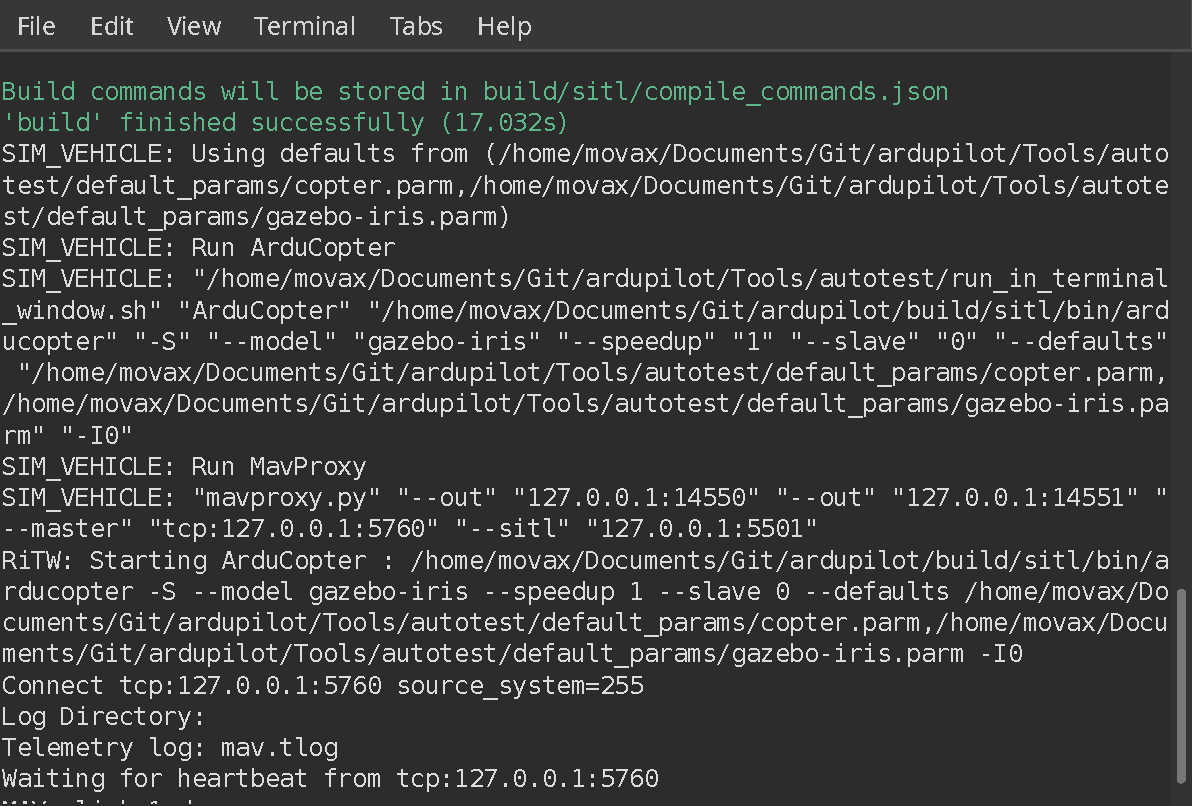
\includegraphics[width=0.7\textwidth]{Ardupilot_Py.pdf}
    \caption{Datos de conexión de ArduPilot}
    \label{fig:Ardupilot_Py}
\end{figure}

Una vez que se entabló la conexión entre ambas partes es posible tener acceso a toda clase de datos de vuelo, entre ellos la actitud del dron. Cabe mencionar que, en los mensajes que recibe Pymavlink por parte de ArduPilot es una trama de datos de gran longitud, y debido a que se creó un objeto de Python para entablar la conexión, es posible acceder a un dato en específico como se accede a un atributo en la instancia de una clase. En este caso, se decidió imprimir en consola el dato del ángulo de roll de dron con el fin de comprobar que la comunicación se dio de forma exitosa. 

Por último con respecto a esta subsección, la figura \ref{fig:pymav_listen} muestra el resultado de haber entablado una comunicación exitosa entre Pymavlink y el piloto automático, en la figura \ref{fig:pymav_atitude} se logra apreciar la trama completa con los datos referentes a la actitud del dron al momento de llevar a cabo la comunicación, mientras que la figura \ref{fig:pymav_roll} presenta esta trama de forma filtrada, de tal manera que solo se imprime el ángulo de roll del dron.
 

\begin{figure}[ht]
    \centering
    \subfloat[Trama de datos de la actitud del dron]{\label{fig:pymav_atitude}{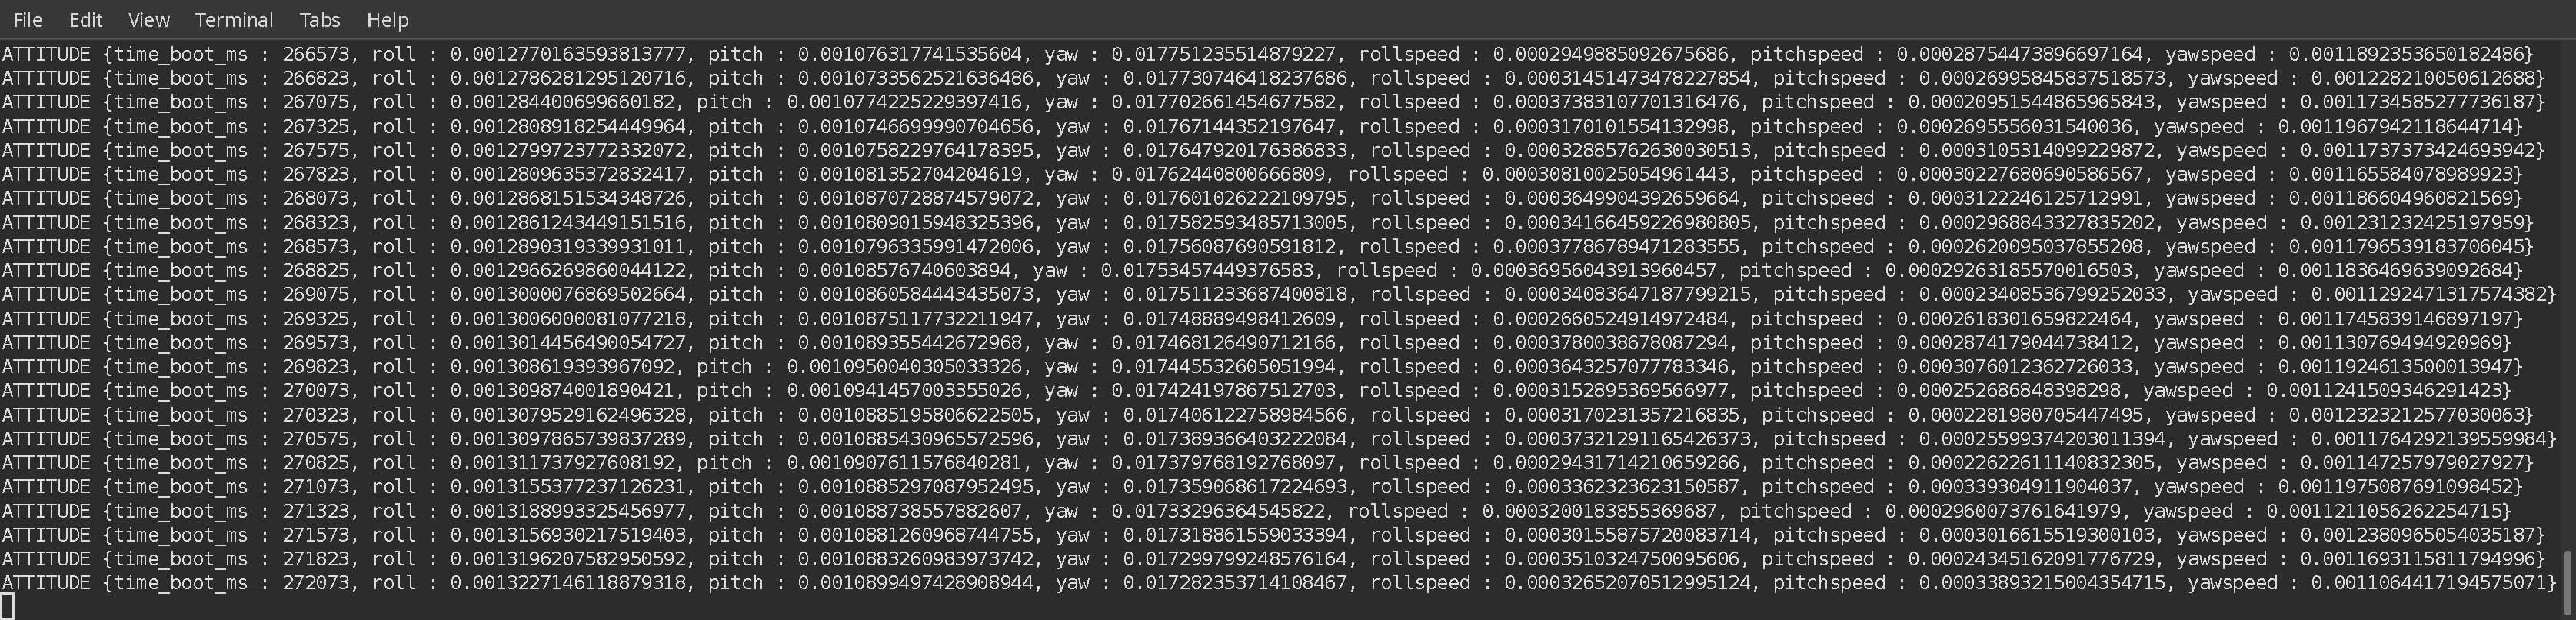
\includegraphics[width=0.95\textwidth]{pymav_atitude.pdf}}}\\
    \subfloat[Datos del roll]{\label{fig:pymav_roll}{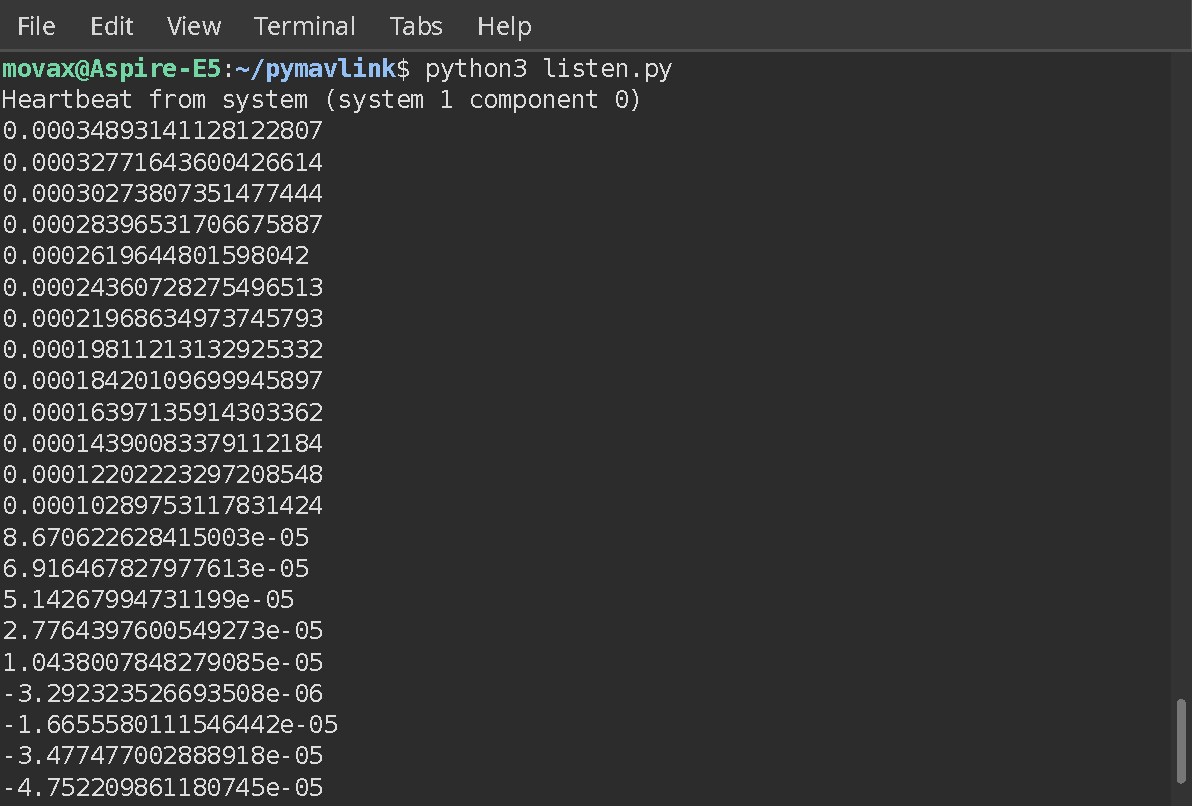
\includegraphics[width=0.4\textwidth]{pymav_roll.pdf}}}
    \caption{Datos obtenidos a partir de la conexión entre ArduPilot y Pymavlink} 
    \label{fig:pymav_listen}
\end{figure}


\section{Configuración de modo de vuelo}

De acuerdo con la documentación oficial de ArduPilot \cite{Ardu_modes}, el Arducopter cuenta con una gran variedad de modos de vuelo, no obstante, en este trabajo solo se utilizan únicamente dos modos, \textit{guided} y \textit{land}; el primero permite enviar comando de vuelo de forma directa al piloto automático a través de mensajes, mientras que el segundo ejecuta una rutina de aterrizaje para el dron. Este último modo de vuelo se aborda en la subsección marcada como extra.

Entonces, previo a la secuencia de despegue del dron, es necesario configurar el modo de vuelo en guided, pues al iniciar el SITL de ArduPilot, este inicializa con el modo de vuelo "stabilize", de tal forma que el piloto automático no es capaz de recibir comandos de vuelo ingresado directamente por el usuario. Esto representa un problema pues se busca que la trayectoria de vuelo del dron sea determinada a partir de un conjunto predefinido de waypoints.

Con base en lo anterior, el script perteneciente a esta subsección busca el identificador perteneciente al modo de vuelo indicado, dentro de una tabla de valores pre-configurados dentro de la librería, y utiliza el objeto de la subsección anterior para enviar el comando de selección de modo de vuelo al piloto automático. En dado caso de que el modo de vuelo especificado tenga un registro válido dentro de la tabla de la librería, se imprime un mensaje en donde se confirma que el modo de vuelo ha sido cambiado.

Por último, el método utilizado para establecer el modo de vuelo fue \textit{set\_mode\_send}, el cual recibe solamente 3 parámetros, el atributo del sistema del objeto de la conexión, el comando para establecer el modo de vuelo, y el código de identificación del modo de vuelo especificado. La figura \ref{fig:pymav_modes} muestra el resultado que se obtuvo al ejecutar el código desarrollado para esta subsección, en la figura \ref{fig:pymav_mode} se observa el mensaje de ejecución del script como tal, y por otro lado, la figura \ref{fig:Ardupilot_mode} presenta la aceptación del comando y el cambio de modo de vuelo reflejado en la terminal de ArduPilot.


\begin{figure}[ht]
    \centering
    \subfloat[Respuesta en Pymavlink]{\label{fig:pymav_mode}{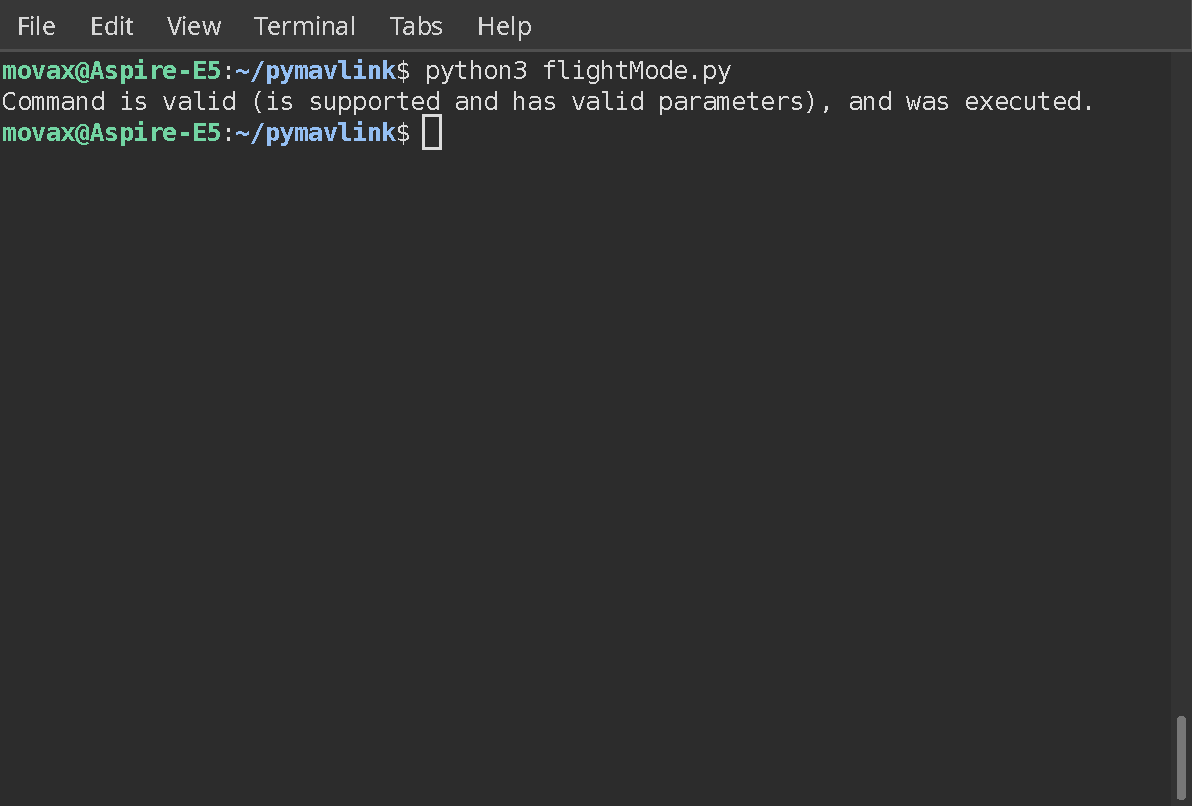
\includegraphics[width=0.48\textwidth]{pymav_mode.pdf}}}\hfill
    \subfloat[Respuesta en ArduPilot]{\label{fig:Ardupilot_mode}{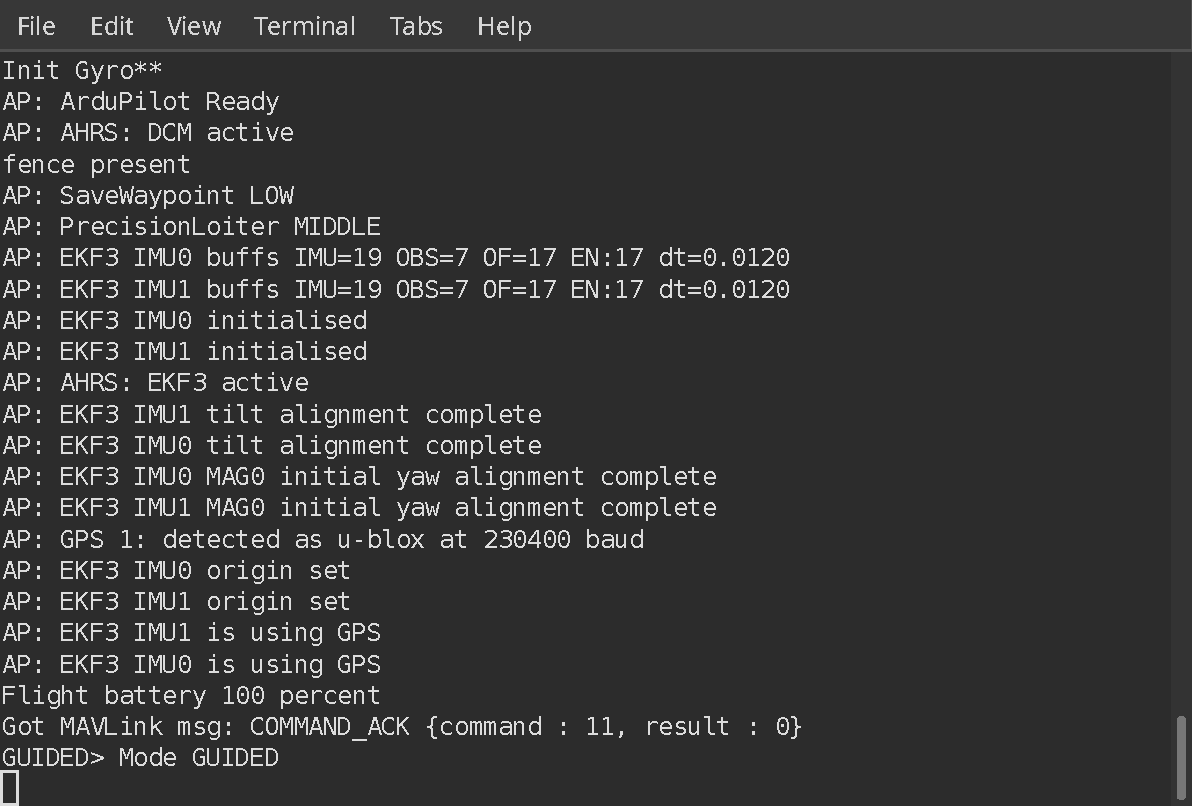
\includegraphics[width=0.48\textwidth]{Ardupilot_mode.pdf}}}
    \caption{Ejecución del script para la configuración del modo de vuelo}
    \label{fig:pymav_modes}
\end{figure}


\section{Secuencia de despegue}

Una vez que se logró entablar la comunicación con el piloto automático y se seleccionó en modo de vuelo adecuado, la secuencia de despegue resulto bastante sencilla de implementar, pues solo consta de dos pasos; enviar el comando para el armado de motores y enviar el comando de despegue especificando la altura deseada. Sin embargo, para que lo anterior se logre ejecutar de manera correcta, es necesario esperar a que los sistemas de la computadora de vuelo se inicialicen por completo, en especial aquellos sensores que sirven para la estimación de posición del dron, pues se requiere de estos para que el dron pueda despegar y elevarse a la altura solicitada por el usuario.

Esto último representó un problema al momento de crear el nodo de la misión de vuelo en ROS, pues si los filtros de estimación no se encuentran listos al momento de ejecutar el comando de despegue, la instrucción no se ejecuta y el dron es incapaz de iniciar su rutina de vuelo. La solución a este problema se aborda en la respectiva sección de ROS.

Dicho lo anterior, el script perteneciente a esta subsección no cuenta con la etapa de la selección del modo de vuelo, pues es necesario ejecutar el programa en el momento en el que los filtros del sistema han sido inicializados, y si se corre el script al mismo tiempo que  se inicia el SITL, el comando de despegue es rechazado. Entonces, para ejecutar el programa, el usuario tiene que cambiar el modo de vuelo de forma manual dentro de la terminal de ArduPilot, de esta forma se asegura que el sistema está listo para recibir la instrucción de despegue.

Además, en este caso el script envía los comandos al piloto automático mediante la instrucción command\_long\_send, la cual recibe 11 parámetros; en donde los primeros 2 corresponden al sistema y al componente de MAVLink, los cuales son atributos pertenecientes al objeto creado al momento de establecer la comunicación con el piloto automático. Por otro lado, el siguiente parámetro corresponde al comando de vuelo que se desea enviar y los siguientes 8 sus respectivos atributos. Recordando que un comando de MAVLink puede recibir hasta 7 atributos, existen muchos comando en donde no se ocupan por completo esta cantidad de atributos, en estos casos, es necesario revisar la documentación perteneciente al comando en cuestión y verificar la cantidad especifica de atributos requeridos, el resto de parámetros no utilizados se debe de dejar en 0.

Entonces, en el caso de esta etapa, los comandos de vuelo utilizados fueron \textit{MAV\_ CMD\_COMPONENT\_ARM\_DISARM} para el armado de los motores y \textit{MAV\_CMD\_NAV\_ TAKEOFF} para la orden de despegue. La figura \ref{fig:pymav_takeoff} muestra el comportamiento observado en la simulación tras la ejecución del script con la secuencia de despegue, la figura \ref{fig:pymav_takeoff1} presenta el estado inicial de la simulación, antes de que se enviara el comando de vuelo, por otro lado, la figura \ref{fig:pymav_takeoff2} muestra el dron en vuelo, tras haber alcanzado la altura indicada en el comando de vuelo. Entonces, a simple vista se logra apreciar que el comando se ejecutó de manera correcta y el dron despega sin ningún tipo de problema.  

\begin{figure}[ht]
    \centering
    \subfloat[]{\label{fig:pymav_takeoff1}{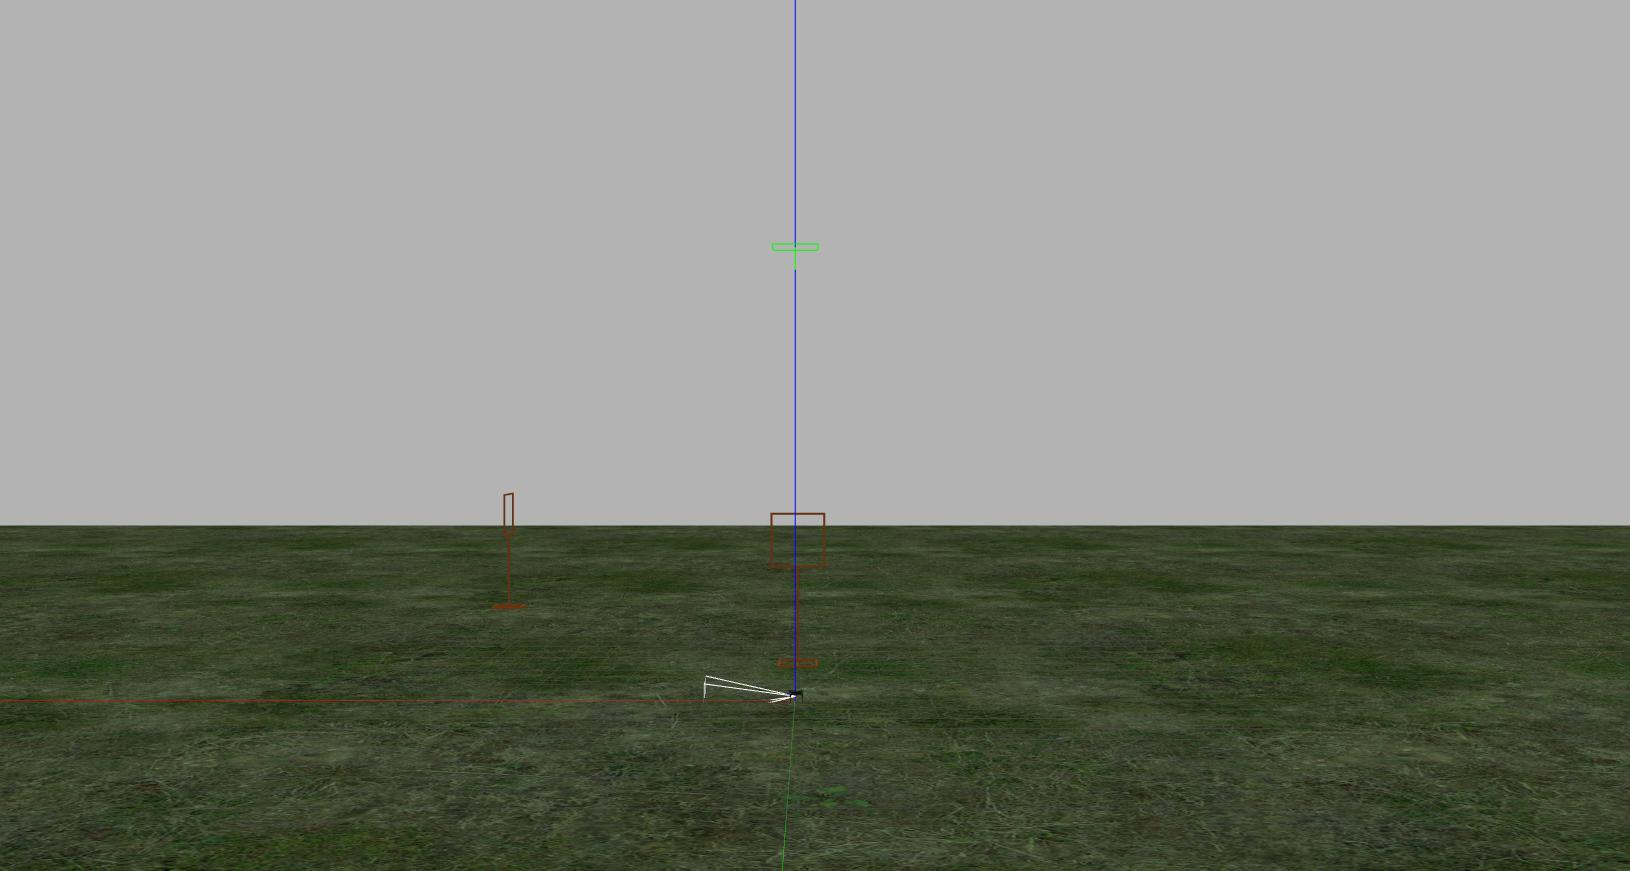
\includegraphics[width=0.48\textwidth]{pymav_takeoff1.jpg}}}\hfill
    \subfloat[]{\label{fig:pymav_takeoff2}{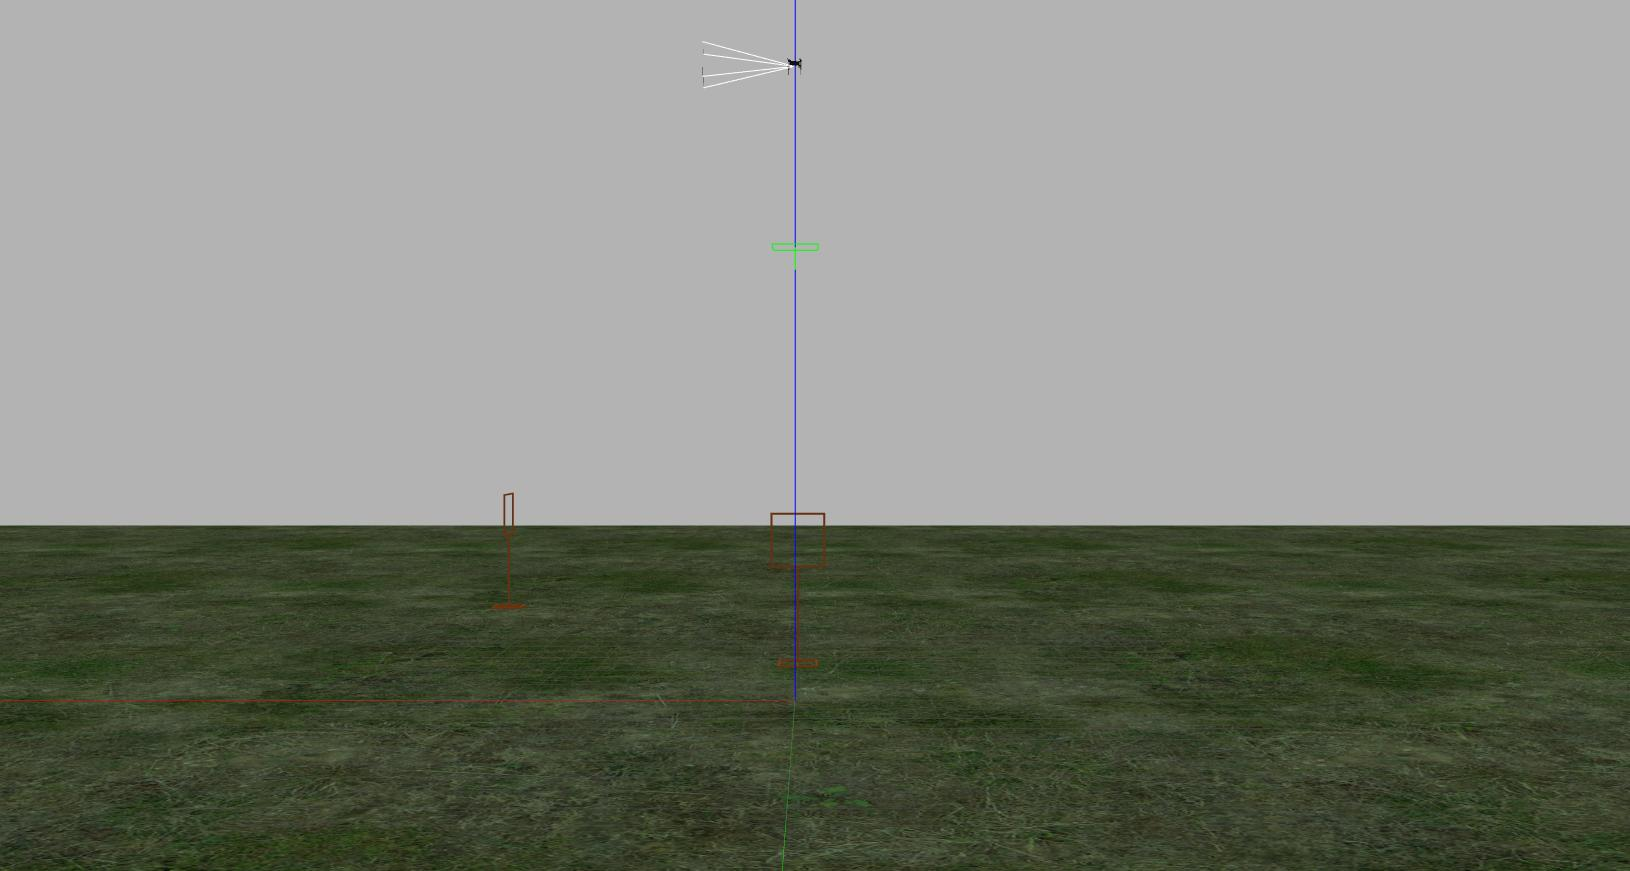
\includegraphics[width=0.48\textwidth]{pymav_takeoff2.jpg}}}
    \caption{Comportamiento de la simulación ante el comando de despegue}
    \label{fig:pymav_takeoff}
\end{figure}


Si bien la figura \ref{fig:pymav_takeoff} muestra de manera acertada la correcta ejecución de la secuencia de despegue, a simple vista resulta difícil decir con exactitud sin el dron alcanzó, o no, la altura desea. Debido a lo anterior, se recopilaron los datos correspondientes a la posición y velocidad del dron durante su ascenso, a partir de uno de los mensajes de MavLink que permite obtener acceso a esta información manejada por el piloto automático. En consecuencia, la figura \ref{fig:pymav_takeoffz} es una gráfica que muestra la altura del dron durante su despegue, de tal forma que es posible apreciar que, en efecto, el dron logra alcanzar la altitud deseada durante su despegue con un ligero sobre paso, aproximadamente a los 13 segundos después de comenzar a ejecutar el comando de vuelo. Por otro lado, cabe mencionar que, debido al marco de referencia con el que se está trabajando, un desplazamiento hacia arriba en el eje \textit{z} es considerado negativo, mientras que un desplazamiento hacia abajo en ese eje se considera positivo; sin embargo, para fines de una interpretación de datos más intuitiva, se invirtió el signo de la lectura de datos en el eje \textit{z}. 

\begin{figure}[h]
    \centering
    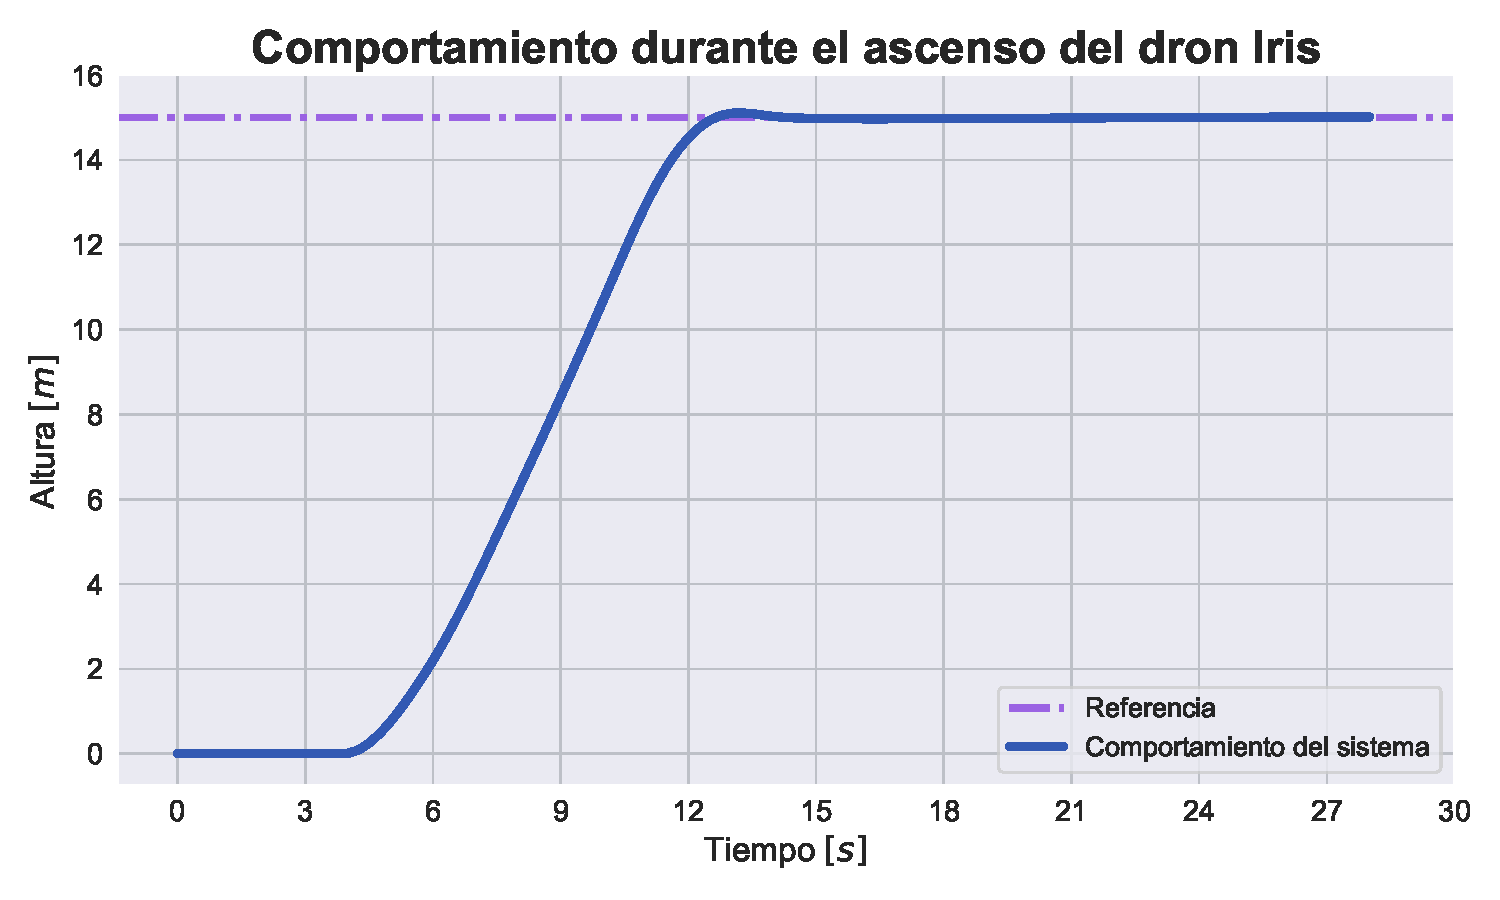
\includegraphics[width=0.7\textwidth]{pymav_takeoffz.pdf}
    \caption{Respuesta en la altura para el comando de despegue.}
    \label{fig:pymav_takeoffz}
\end{figure}

Adicionalmente, la figura \ref{fig:pymav_takeoffvz} corresponde a una gráfica que describe el comportamiento de la velocidad de ascenso del dron, y de manera congruente con la gráfica mencionada anteriormente, se puede apreciar un descenso en la velocidad de ascenso en el intervalo de tiempo de 10 s y 15 s, lapso en el que el dron logra llegar a la referencia y por lo tanto ya no es necesario ascender más;  además, se observa una velocidad máxima de ascenso de 2.21 $\frac{m}{s}$.

\begin{figure}[ht]
    \centering
    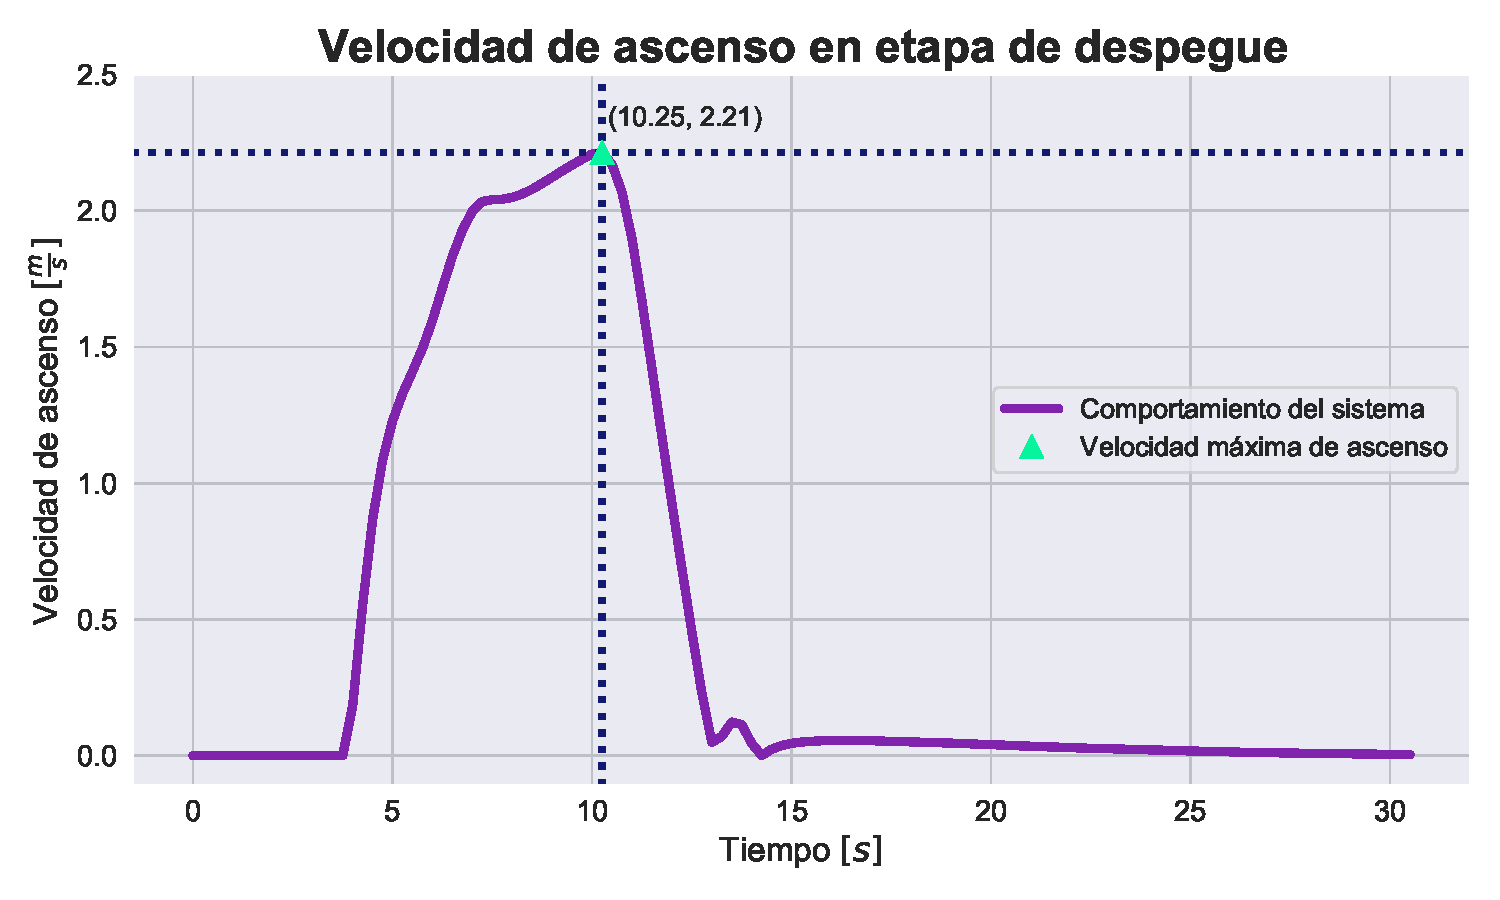
\includegraphics[width=0.7\textwidth]{pymav_takeoffvz.pdf}
    \caption{Gráfica de velocidad de despegue.}
    \label{fig:pymav_takeoffvz}
\end{figure}

\section{Seguimiento de trayectoria}

Hecho todo lo anterior, la última prueba que se tuvo que realizar, en cuanto a una funcionalidad en específico de Pymavlink, fue la del seguimiento de trayectoria por medio de comandos de vuelo directos, en forma de waypoints. Sin embargo, debido al problema mencionado en la etapa anterior, el script perteneciente a esta subsección no ejecuta las etapas anteriores, sino que para poder ejecutar el programa, el usuario tiene que esperar a que la terminal de Ardupilot permita el cambio de modo de vuelo de forma manual, y después ejecutar los respectivos comandos de vuelo para realizar la secuencia de despegue del dron.

Ahora bien, la prueba realizada para esta etapa fue sencilla, se enviaron dos waypoint utilizando el marco de referencia local, en donde el origen, o la coordenada (0,0,0), corresponde al punto inicial del mundo creado, denotado de forma visual por 3 barras ortogonales de color azul para el eje \textit{z}, azul para el eje \textit{x} y verde para el eje \textit{y}. Además, como se mencionó, la trayectoria de vuelo está compuesta por dos waypoints, los cuales fueron definidos de tal manera que se buscó que el dron cruzara por las dos primeras compuertas del circuito de vuelo, dichos waypoint son [35,0,3] y [35, 17, 2]; Dicho esto, la secuencia pensada para la ejecución de esta prueba fue, primero hacer ascender el dron a una altura de 10 m y después indicarle su trayectoria de vuelo a partir de los waypoints especificados. 

Asimismo, se buscó comprobar si el piloto automático espera a que el dron llegue al primer waypoint para dirigirse hacía el segundo, sin embargo, esto no sucede y el piloto automático ejecuta el segundo waypoint definido, pues no hay ningún tiempo de espera o bandera que le indique al piloto que debe de esperar a que se termine la ejecución del primer waypoint. Entonces, para evitar que el piloto automático ignorara el primer waypoint, se utilizó un mensaje de MAVLink definido como \textit{NAV\_CONTROLLER\_OUTPUT} el cual publica información relacionada sobre el comando de vuelo enviado al piloto automático, entre la cual se encuentra la distancia faltante para que el dron llegue al waypoint especificado al momento de lectura del mensaje. Entonces, la instrucción para el seguimiento del segundo waypoint es enviada al piloto automático hasta que el mensaje especifica que la distancia restante para llegar al primer waypoint es igual a cero.

Continuando con los resultados de la prueba, en este caso el script solo ejecuta las instrucciones para guiar el vuelo del dron, por lo que es necesario que el usuario realice todo el pre-proceso necesario para el despegue del dron. En el caso de la prueba realizada la altitud de despegue indicada fue de 10 m, por lo que para el seguimiento del waypoint, el dron tuvo que descender a 3 m de altura al mismo tiempo que avanzó 10 m en el eje x, y después otros 20 m. Cabe mencionar que para el piloto automático, una altura negativa indica un punto sobre la referencia inicial, y análogamente, una altura positiva corresponde a un punto por debajo de la referencia inicial. 

Además, los waypoints son enviados utilizando el comando de vuelo \textit{MAVLink\_set\_ position\_target\_local\_ned\_message}, el cual requiere 16 parámetros para realizar el seguimiento de un waypoint. La tabla \ref{tab:waypoint} enlista los parámetros y muestra una breve descripcción de los mismos; Por otro lado, el parámetro type\_mask  es algo complejo de explicar, por lo que, por motivos de practicidad y legibilidad, se describe a más detalle fuera de la tabla.

Retomando lo anterior, el parámetro type\_mask indica la cantidad de parámetros que el comando de vuelo tiene que tomar en cuenta de acuerdo a lo que el usuario desee indicar, dígase posición, velocidad, aceleración o las tres magnitudes anteriores. Dicho esto, mencionando un ejemplo, si se desea enviar un comando de velocidad, es necesario especificar la velocidad de referencia para los 3 ejes cartesianos y el resto de parámetros serán ignorados independiente del valor indicado en el comando.

Adicionalmente, la tabla \ref{tab:waypoint_mask} muestra los distintos valores que se le pueden asignar al parámetro de máscara. En el caso de este trabajó se utilizó el primer tipo de máscara, debido a que solo se buscó que el dron siguiera una trayectoria, con la máxima velocidad que el vehículo pudiera proporcionar.

\begin{table}[ht]
    \centering
    \begin{tabular}{ll}
        \hline
        Parámetro & Descripción\\
        \hline
        \hline
        time\_boot\_ms & Tiempo de arranque del sistema en ms\\
        target\_system & Identificador del sistema\\
        target\_component & Identificador del componente o controlador de vuelo\\
        coordinate\_frame & Marco de referencia\\
        type\_mask & Indica los campos que se deben de ignorar\\
        x & Posición en el eje \textit{x} en m\\
        y & Posición en el eje \textit{y} en m\\
        z & Posición en el eje \textit{z} en m\\
        vx & Velocidad en el eje \textit{x} en m/s\\
        vy & Velocidad en el eje \textit{y} en m/s\\
        vz & Velocidad en el eje \textit{z} en m/s\\
        afx & Aceleración en el eje \textit{x} en m/$s^2$\\
        afy & Aceleración en el eje \textit{y} en m/$s^2$\\
        afz & Aceleración en el eje \textit{z} en m/$s^2$\\
        yaw & Ángulo de guiñada en radianes\\
        yaw rate & Aceleración de la guiñada en rad/s\\
        \hline
        \hline
    \end{tabular}
    \caption{Parámetros de la instrucción para seguimiento de waypoints}
    \label{tab:waypoint}
\end{table}

\begin{table}[ht]
    \centering
    \begin{tabular}{llll}
        \hline
        Tipo & Binario & Hexadecimal & Decimal\\
        \hline
        \hline
        Posición & 0b110111111000 & 0x0DF8  & 3576 \\
        Velocidad & 0b110111000111 & 0x0DC7  & 3527\\
        Aceleración & 0b110000111111 & 0x0C3F & 3135 \\
        Pos + Vel & 0b110111000000 & 0x0DC0 & 3520\\  
        Pos + Vel + Acel & 0b110000000000 & 0x0C00 & 3072\\
        Guiñada & 0b100111111111 &  0x09FF & 2559\\
        Velocidad de  guiñada& 0b010111111111  & 0x05FF & 1535\\
        \hline
        \hline
    \end{tabular}
    \caption{Tipos de máscara para el comando de seguimiento de trayectoria}
    \label{tab:waypoint_mask}
\end{table}

Ahora bien, retomando el contexto de los resultados obtenidos al momento de ejecutar el script desarrollado para esta subsección, 
la figura \ref{fig:pymav_movement} presenta el comportamiento observado en la simulación tras la ejecución de la secuencia de comando especificada para esta subsección. Entonces, en la figura \ref{fig:pymav_movement1} se observa el estado inicial del dron, previo a la ejecución del protocolo; la figura \ref{fig:pymav_movement2} muestra el dron después de haber ascendido a la altura de 10 m (la cual fue comandada de forma manual a través de la terminal de ArduPilot); Por otro lado, pese a que se mencionó que los waypoints se definieron con el fin de que el dron fuera capaz de cruzar las primeras dos compuertas del circuito de vuelo, en la figura \ref{fig:pymav_movement3} se aprecia que el dron sobrevuela la primera compuerta del circuito y no para a través de ella, esto se debe a la altura de ascenso que se definió durante la prueba, sin embargo, cabe mencionar que si al dron se le comanda un despegue de 3 m (altura a la que se encuentra el centro de las compuertas grandes), este es capaz de cruzar por el centro de las dos primeras compuertas utilizando los dos waypoints definidos; asimismo, la figura \ref{fig:pymav_movement4} muestra una captura del dron después de que este llegó a su punto final tras seguir el segundo waypoint, se aprecia que en este caso el dron si fue capaz de cruzar a través de la segunda compuerta.

\begin{figure}[ht]
    \centering
    \subfloat[]{\label{fig:pymav_movement1}{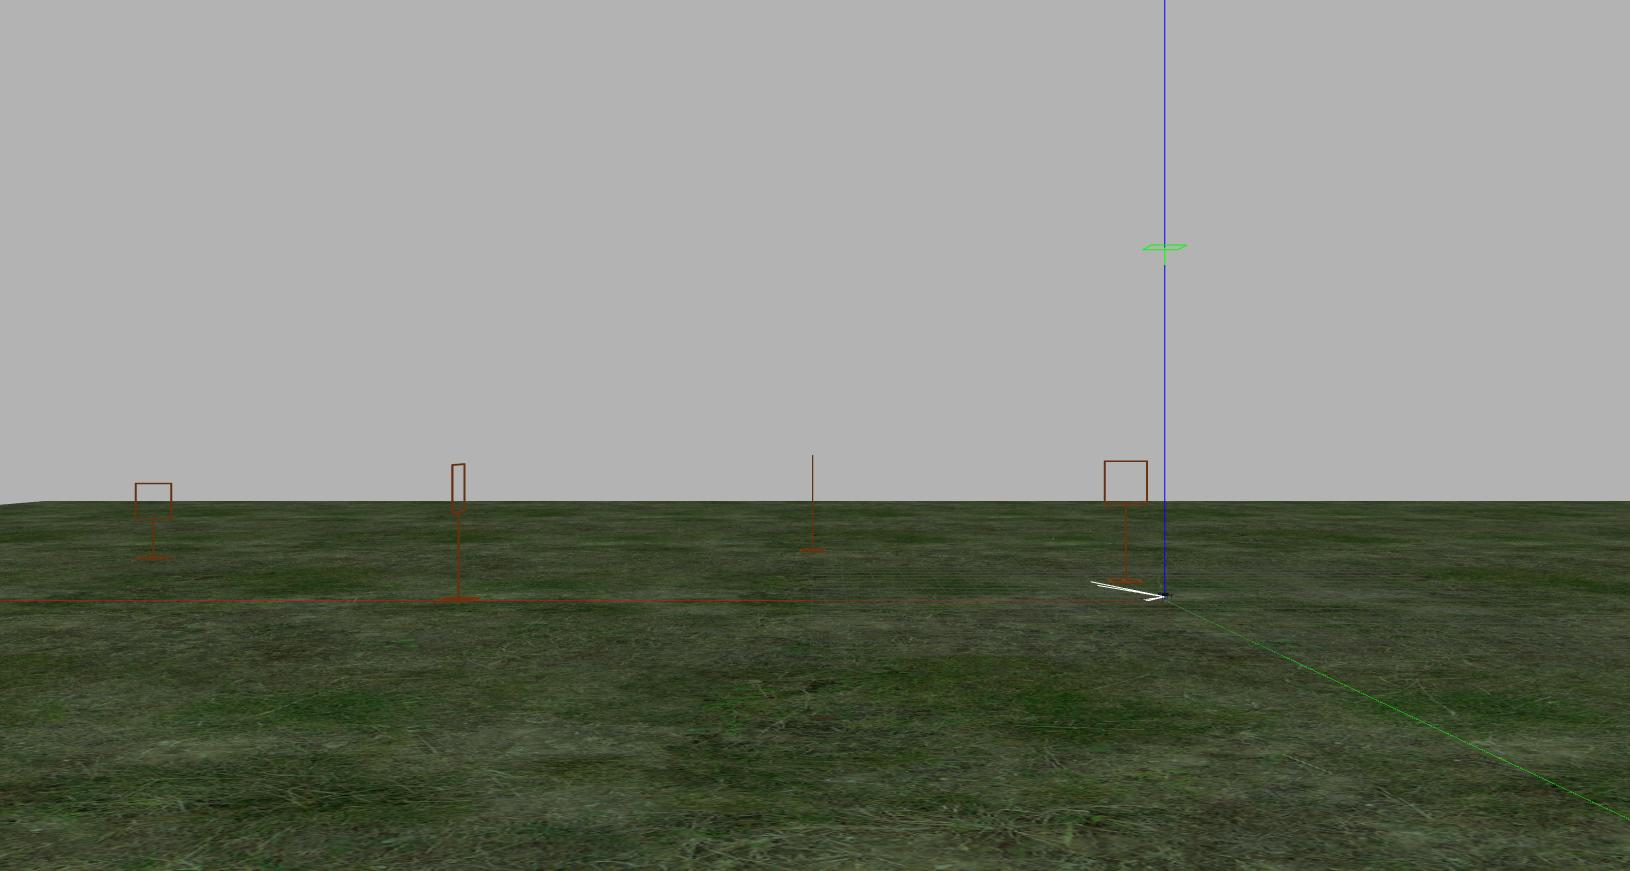
\includegraphics[width=0.48\textwidth]{pymav_movement1.jpg}}}\hfill
    \subfloat[]{\label{fig:pymav_movement2}{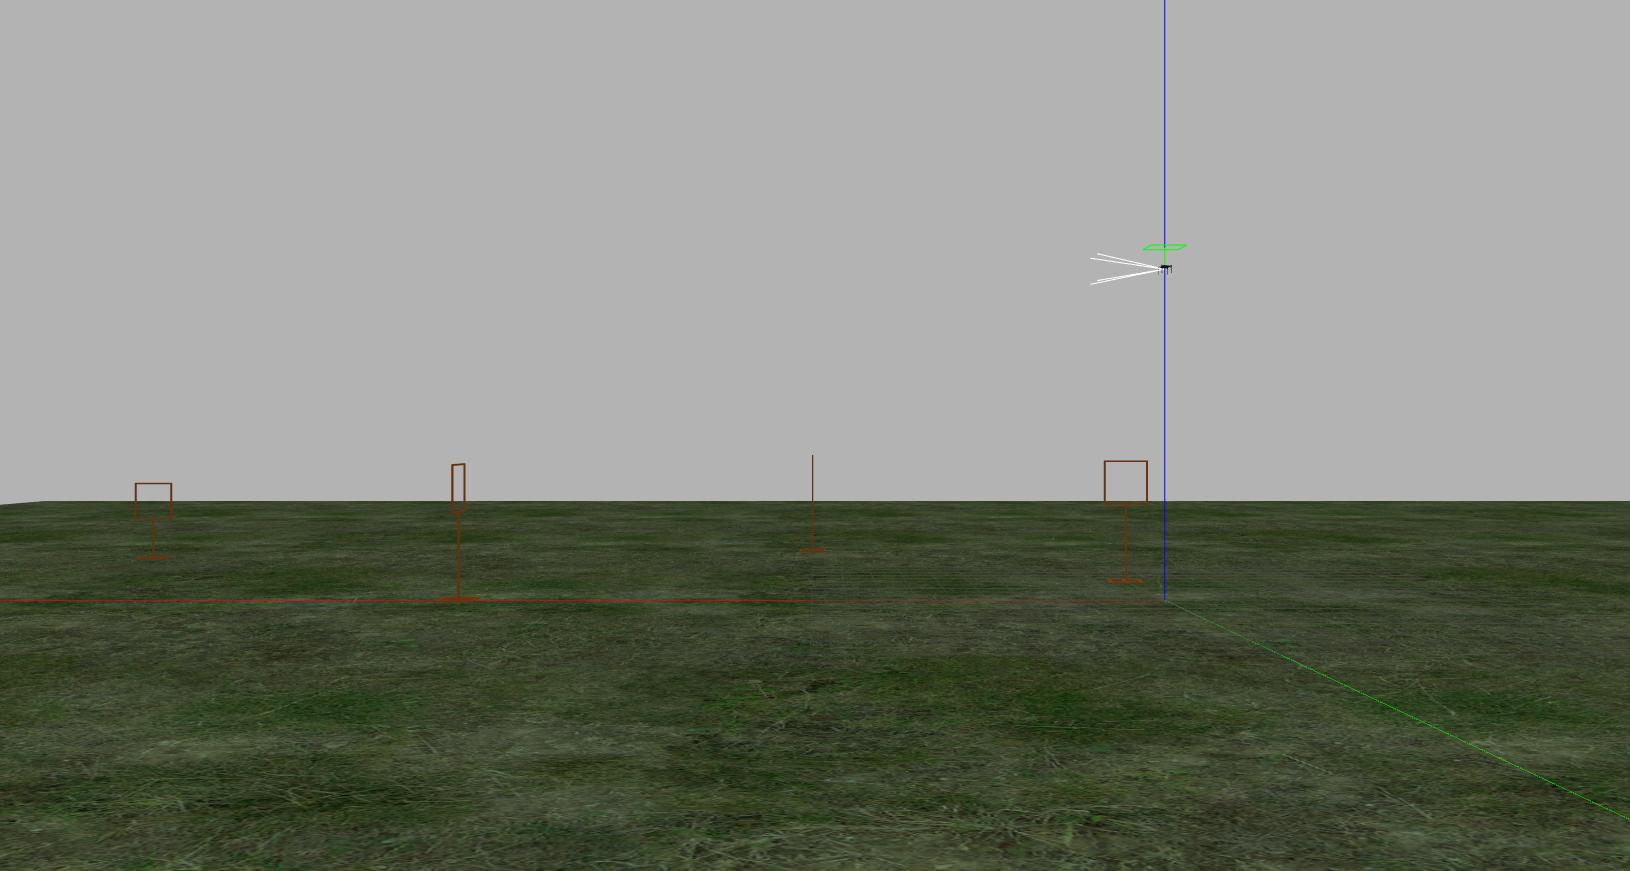
\includegraphics[width=0.48\textwidth]{pymav_movement2.jpg}}}\\
    \subfloat[]{\label{fig:pymav_movement3}{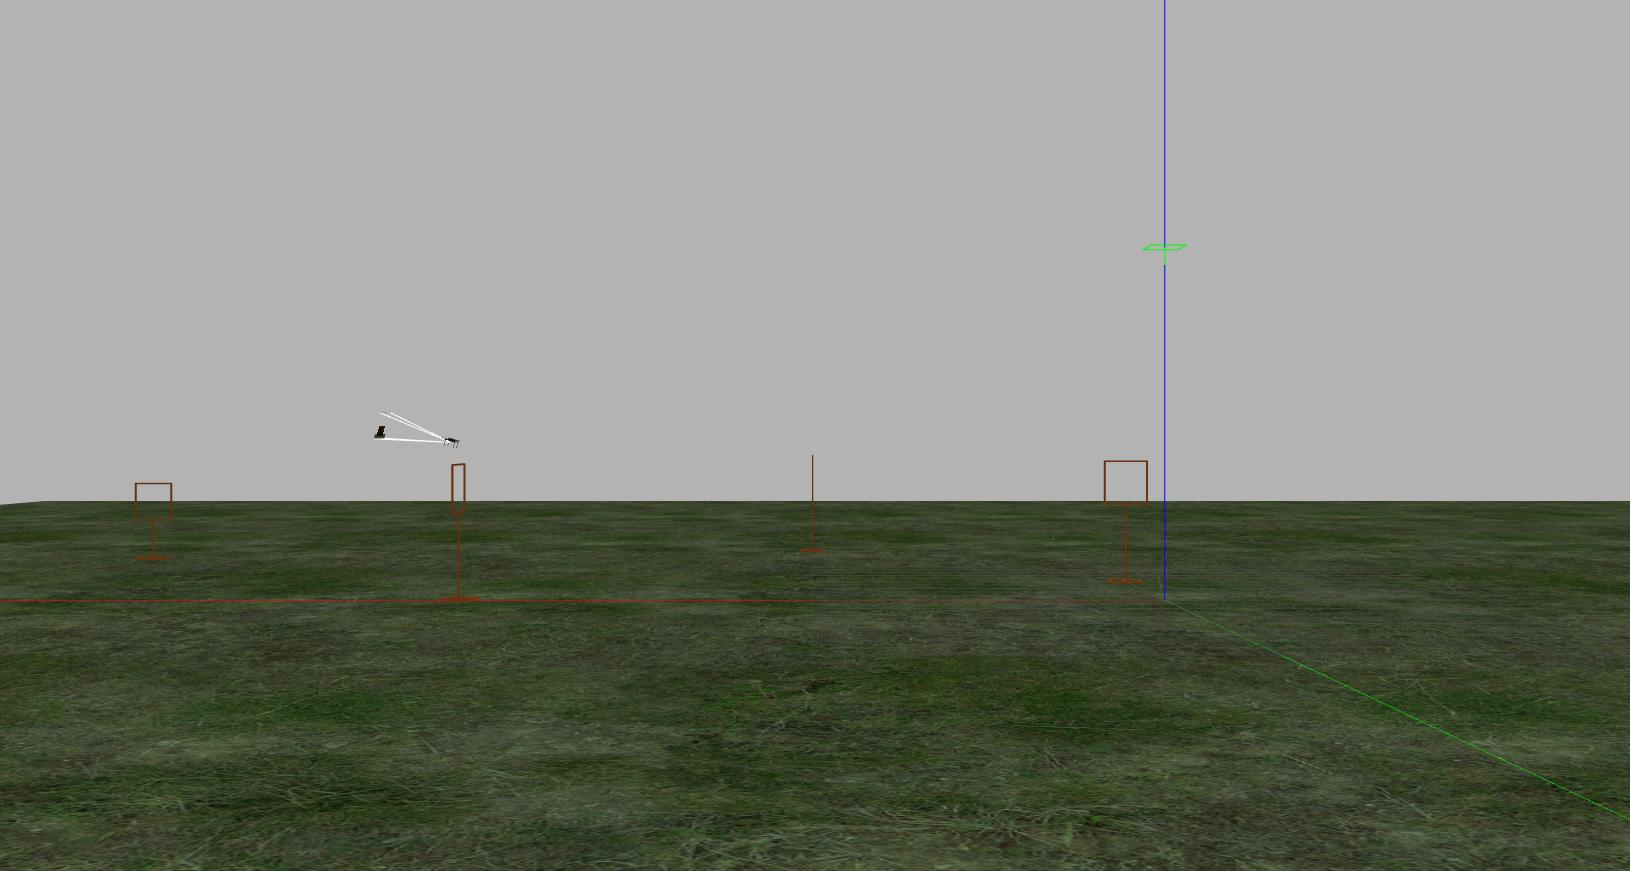
\includegraphics[width=0.48\textwidth]{pymav_movement3.jpg}}}\hfill
    \subfloat[]{\label{fig:pymav_movement4}{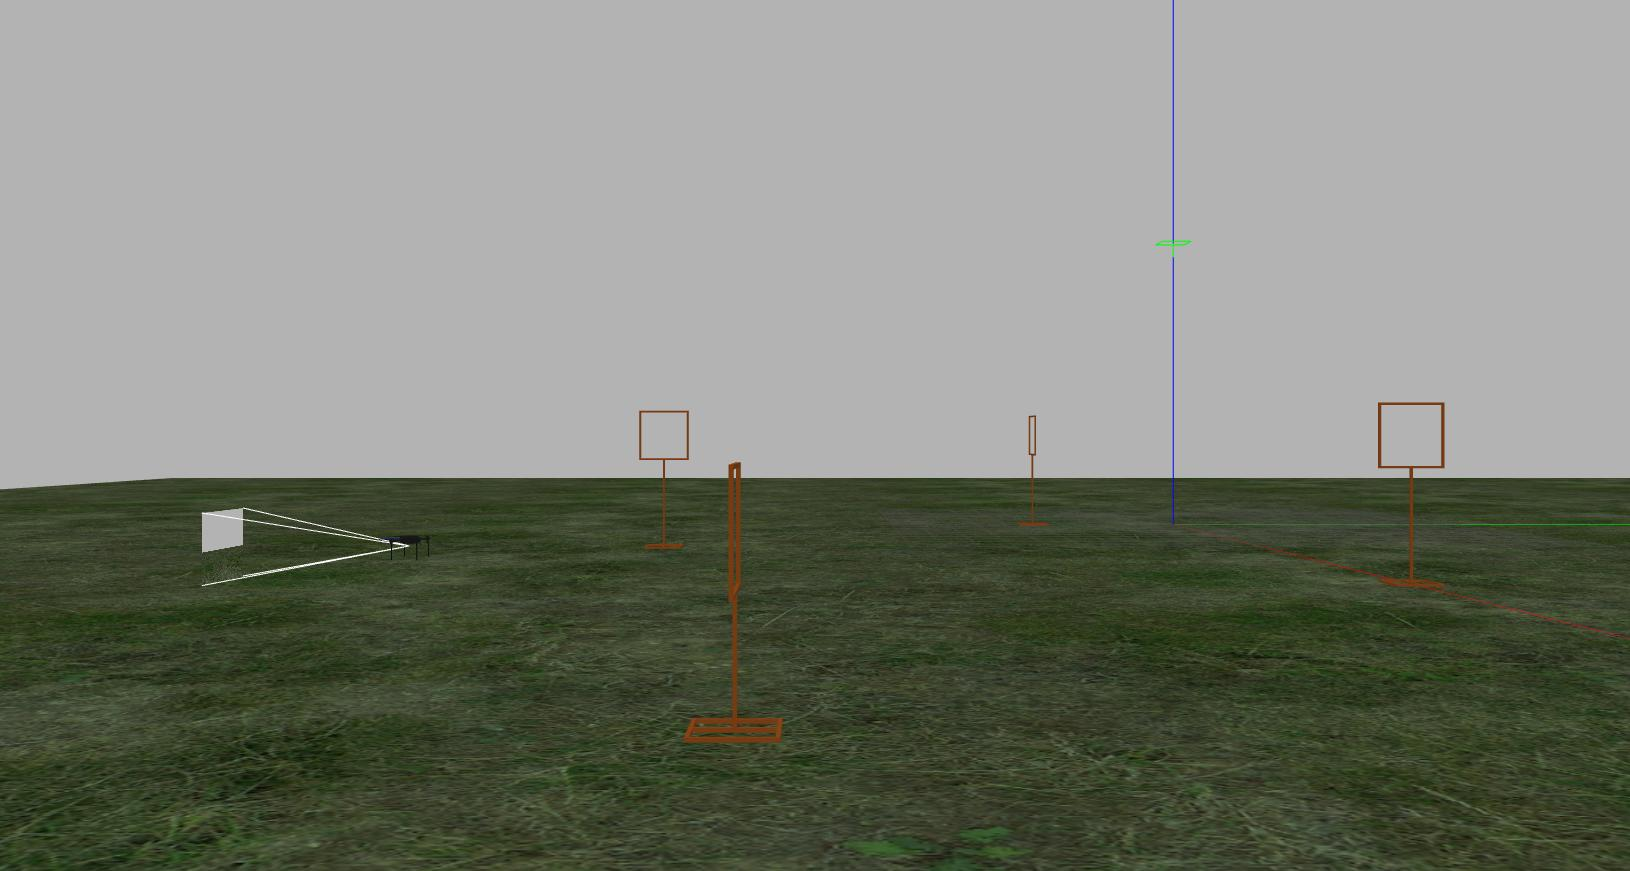
\includegraphics[width=0.48\textwidth]{pymav_movement4.jpg}}}\hfill

    \caption{Etapas de la prueba de seguimiento de trayectoria}
    \label{fig:pymav_movement}
\end{figure}

De manera similar a la subsección anterior, la figura \ref{fig:pymav_movement} permite observar de manera rápida y práctica si el comportamiento del dron fue el adecuado; sin embargo, el análisis del desempeño del dron se logra a partir de los datos de vuelo recopilados. La figura \ref{fig:pymav_movementxy} muestra una gráfica en donde se describe la trayectoria de vuelo seguida por el dron, en ella se especifica la ubicación de las compuertas con base en el recorrido descrito. Cabe mencionar que, contrario a lo que se considera intuitivo, el desplazamiento a lo largo del eje \textit{x} se observa en el eje vertical, mientras que el desplazamiento en el eje \textit{y} corresponde al eje horizontal, esto es debido a que de esta forma la gráfica es congruente con la perspectiva de la cámara dentro de la simulación. En consecuencia, se puede decir que, a partir de la figura \ref{fig:pymav_movementxy}, el dron siguió los waypoints de manera satisfactoria, logrando completar una ruta de vuelo simple. 

\begin{figure}[ht]
    \centering
    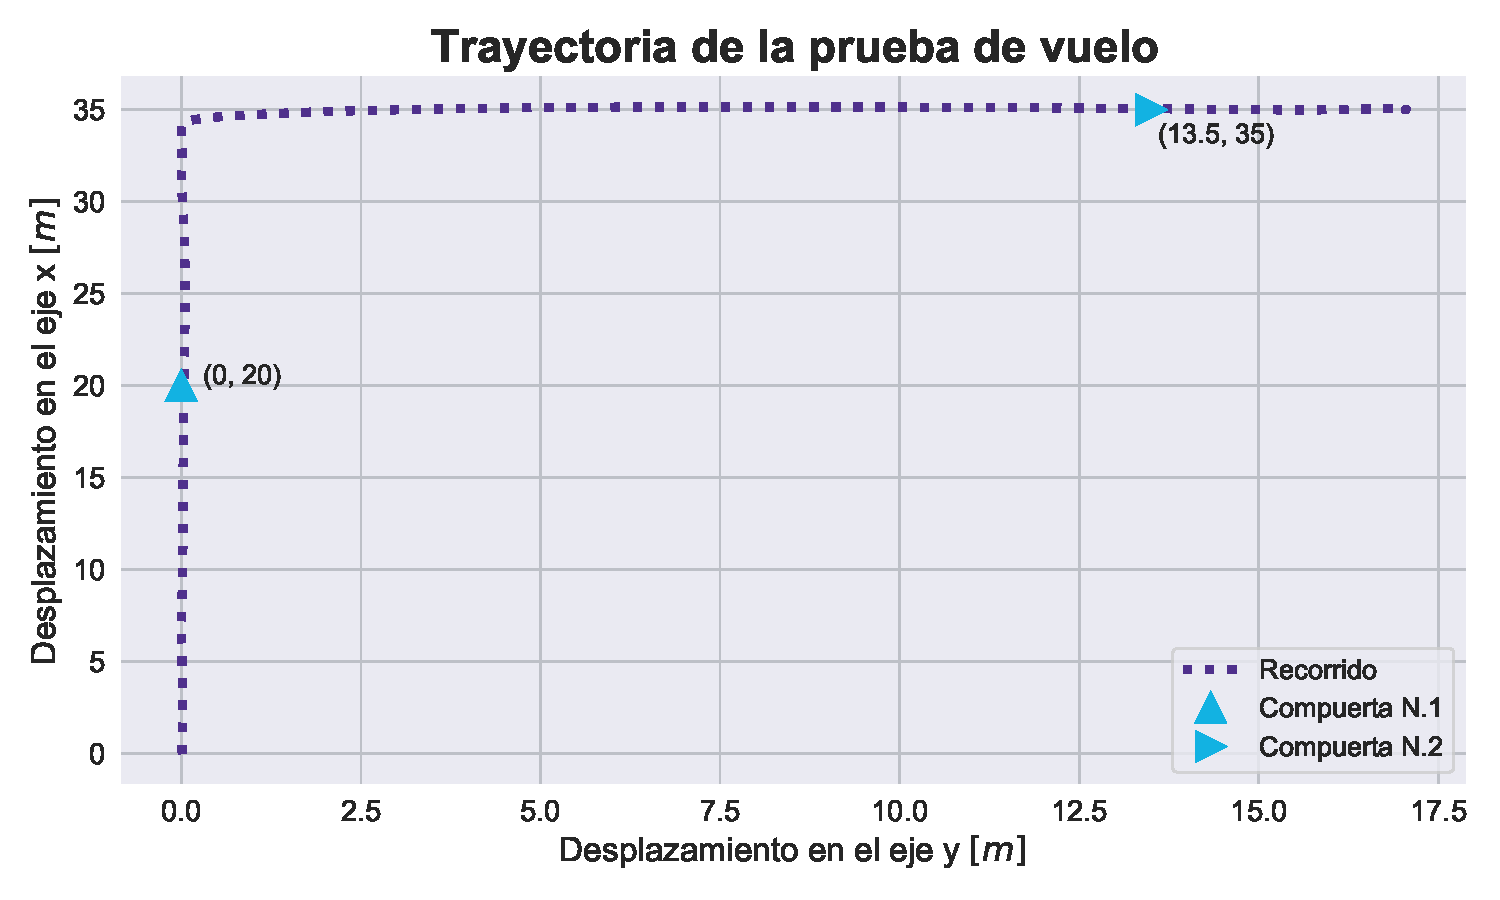
\includegraphics[width=0.8\textwidth]{pymav_movementxy.pdf}
    \caption{Recorrido realizado por el dron}
    \label{fig:pymav_movementxy}
\end{figure}

De forma subsecuente, la figura \ref{fig:pymav_movementd} presenta el comportamiento del desplazamiento lineal del dron a lo largo de los tres ejes espaciales. La figura \ref{fig:pymav_movementx} corresponde al desplazamiento en el eje \textit{x}, en ella se observa como es que el dron llega a la referencia de 35 m sin ningún sobre paso, en un tiempo de aproximadamente 10 s; una vez que el dron completa la trayectoria definida por el primer waypoint, este gira a la izquierda para dirigirse al segundo waypoint, de tal forma que ya no se observa un desplazamiento en el eje \textit{x}, sino, en el eje \textit{y}, en consecuencia, el desplazamiento observado en la gráfica de la figura \ref{fig:pymav_movementy} ocurre hasta el segundo 10, que es cuando se da la transición entre waypoints. Por último, en la gráfica de la figura \ref{fig:pymav_movementz} se logra apreciar el cambio de altura durante el vuelo del dron, resulta evidente la forma en la que el dron desciende de los 10 m indicados en su despegue a una primera referencia de 3 m, y posteriormente el lapso de transición entre waypoints desciende 1 m más, pues la segunda compuerta es más pequeña y está más cerca del suelo; en ambos casos logra el dron logra llegar a la altura indicada.

\begin{figure}[ht]
    \centering
    \subfloat[Eje X]{\label{fig:pymav_movementx}{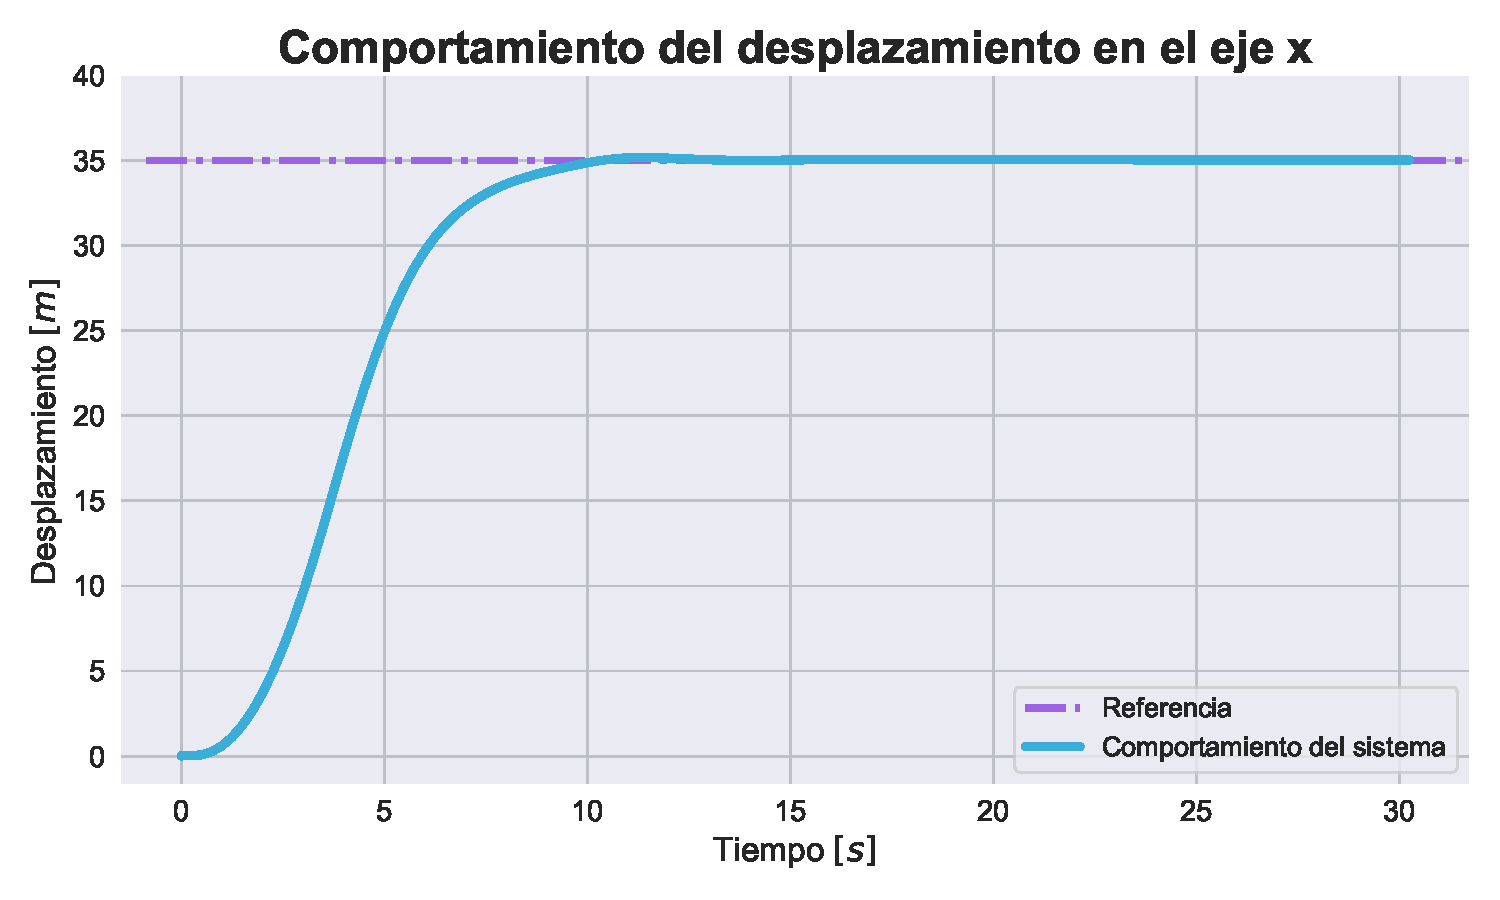
\includegraphics[width=0.48\textwidth]{pymav_movementx.pdf}}}\hfill
    \subfloat[Eje Y]{\label{fig:pymav_movementy}{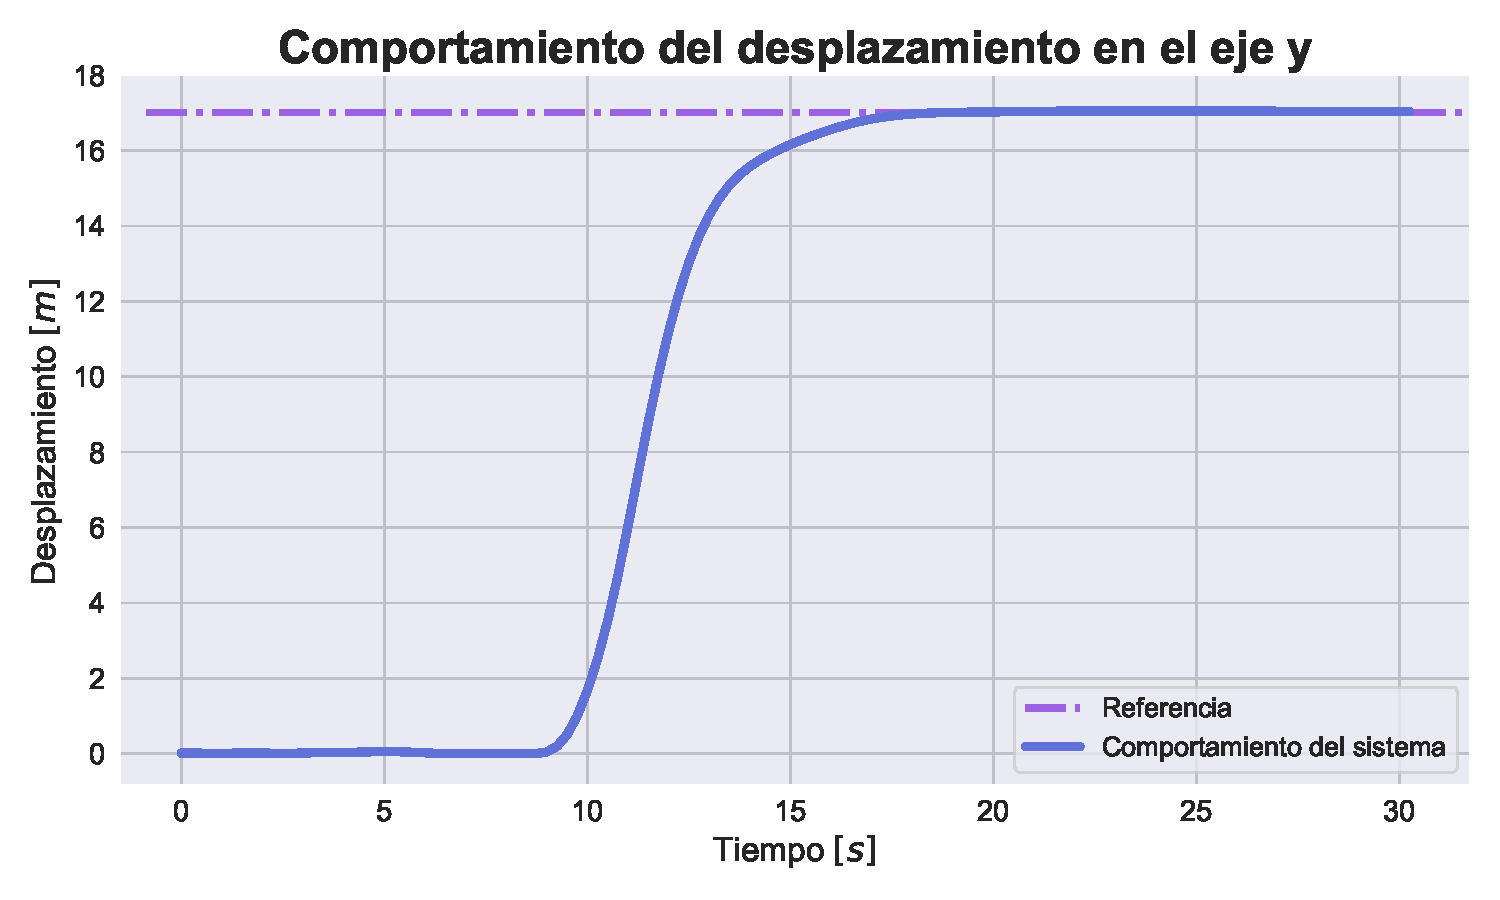
\includegraphics[width=0.48\textwidth]{pymav_movementy.pdf}}}\\
    \subfloat[Eje Z]{\label{fig:pymav_movementz}{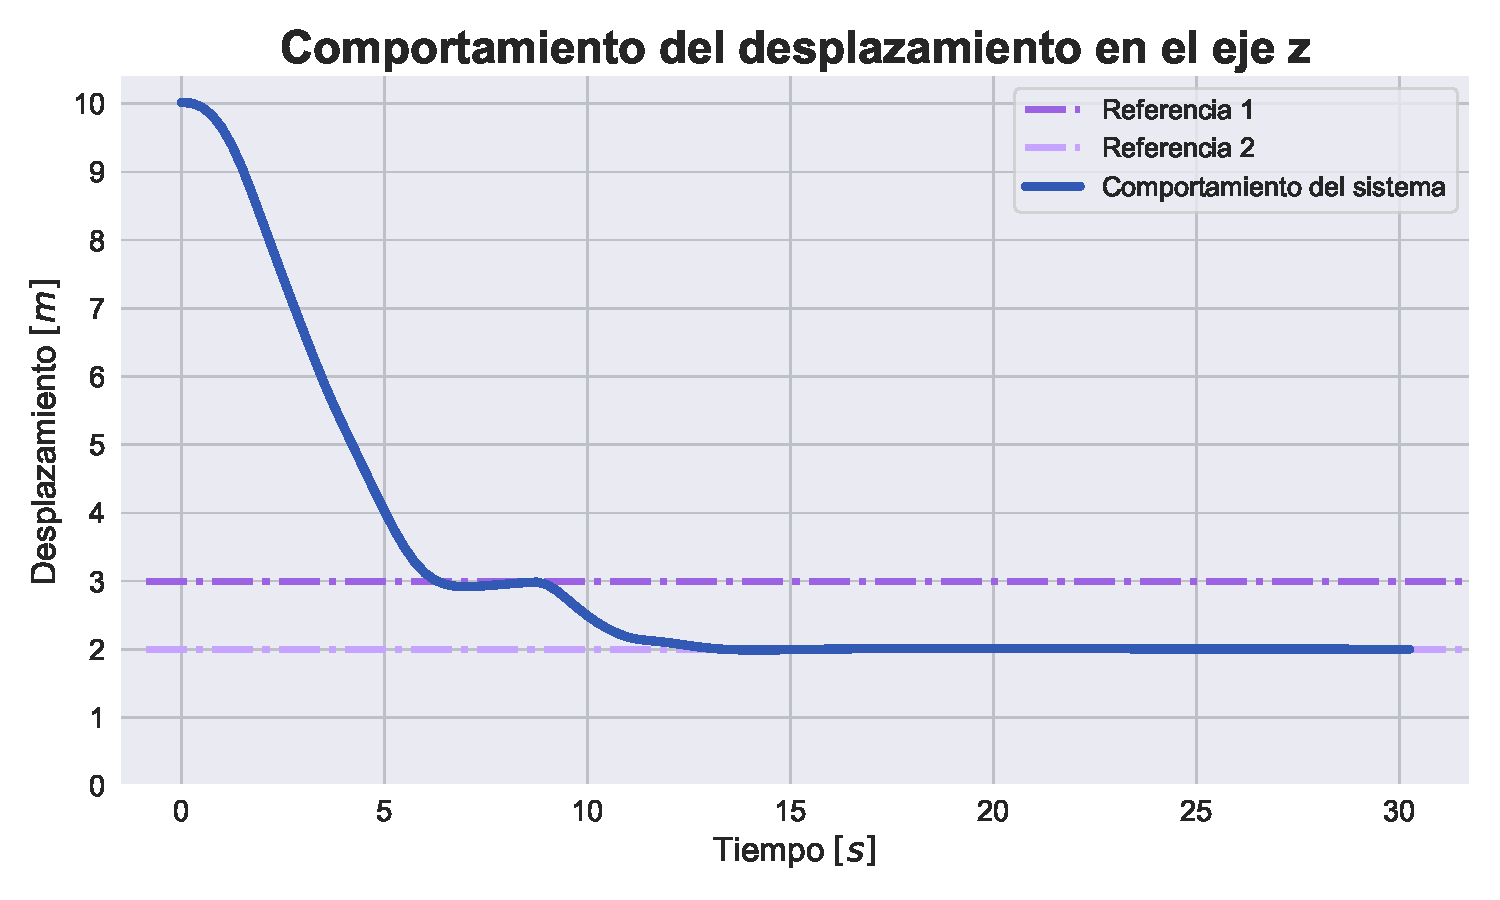
\includegraphics[width=0.48\textwidth]{pymav_movementz.pdf}}}\hfill

    \caption{Gráficas de desplazamiento para los tres ejes}
    \label{fig:pymav_movementd}
\end{figure}

Asimismo, el conjunto de gráficas en la figura \ref{fig:pymav_movementv}, esta esta relacionada con las velocidades lineales asociadas a cada uno de los 3 ejes de desplazamiento del dron. Dicho lo anterior, en la figura \ref{fig:pymav_movementvx}, se observa como en el eje \textit{x} se alcanza la velocidad máxima de 8.34 $\frac{m}{s}$, en el segundo 3.75, antes del tiempo de transición de waypoints, de tal manera que para el segundo 10, la velocidad a lo largo de este eje ha decrecido de forma significativa y de forma intuitiva, se aprecia en la figura \ref{fig:pymav_movementvy} que como es que la velocidad a lo largo del eje \textit{y} comienza su ascenso a partir del tiempo de transición de waypoints, llegando un máximo de 5.59 $\frac{m}{s}$ en el segundo 11.25 del vuelo del dron. 

Por otra parte, la figura \ref{fig:pymav_movementvz} muestra el comportamiento de la velocidad a lo largo del eje \textit{z}; es importante no perder de vista que, como se mencionó en la subsección de la etapa de despegue, los signos de las velocidades fueron invertidos para que el análisis de resultados correspondiera de forma visual con el comportamiento observado durante la ejecución de la simulación. Dicho esto, en la figura \ref{fig:pymav_movementvz} se destaca una pendiente negativa en los primeros 2 segundos de la simulación, esto se debe a que el dron inició a una altura de 10 m y tuvo que descender a 3 m, por lo que el sentido del vector de velocidad fue hacia abajo, llegando a una velocidad de -1.56 $\frac{m}{s}$ en el segundo 2, después de este lapso, el dron tuvo que disminuir su velocidad pues se fue aproximando cada vez más a la altura deseada de 3 m, lo cual ocurrió poco después del segundo 5, con base en la figura \ref{fig:pymav_movementz}; en la gráfica se puede observar un pequeño sobrepaso con una velocidad positiva de 0.0634 $\frac{m}{s}$. Luego, un poco antes del segundo 10, ocurre la transición al siguiente waypoint, por lo que el dron tuvo que descender a los 2 m de altura, una vez más, presentando una velocidad negativa para después detenerse de forma gradual hasta llegar a la altura de referencia. Por último, se observa que el dron finaliza con su recorrido aproximadamente en el segundo 15, pues la velocidad se mantiene en cero después de ese punto.

\begin{figure}[ht]
    \centering
    \subfloat[Eje X]{\label{fig:pymav_movementvx}{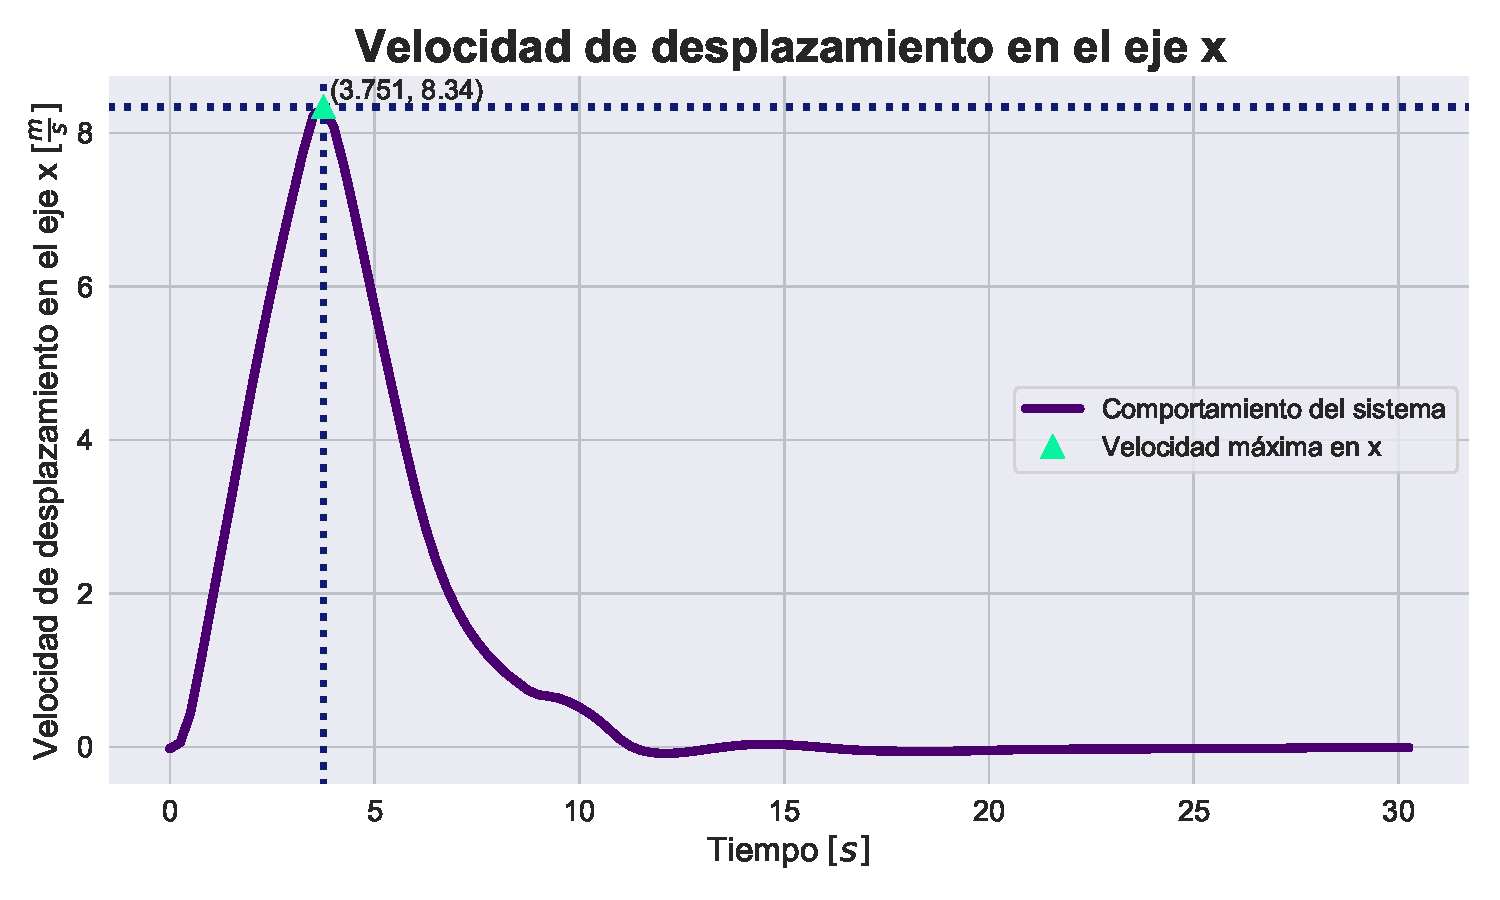
\includegraphics[width=0.48\textwidth]{pymav_movementvx.pdf}}}\hfill
    \subfloat[Eje Y]{\label{fig:pymav_movementvy}{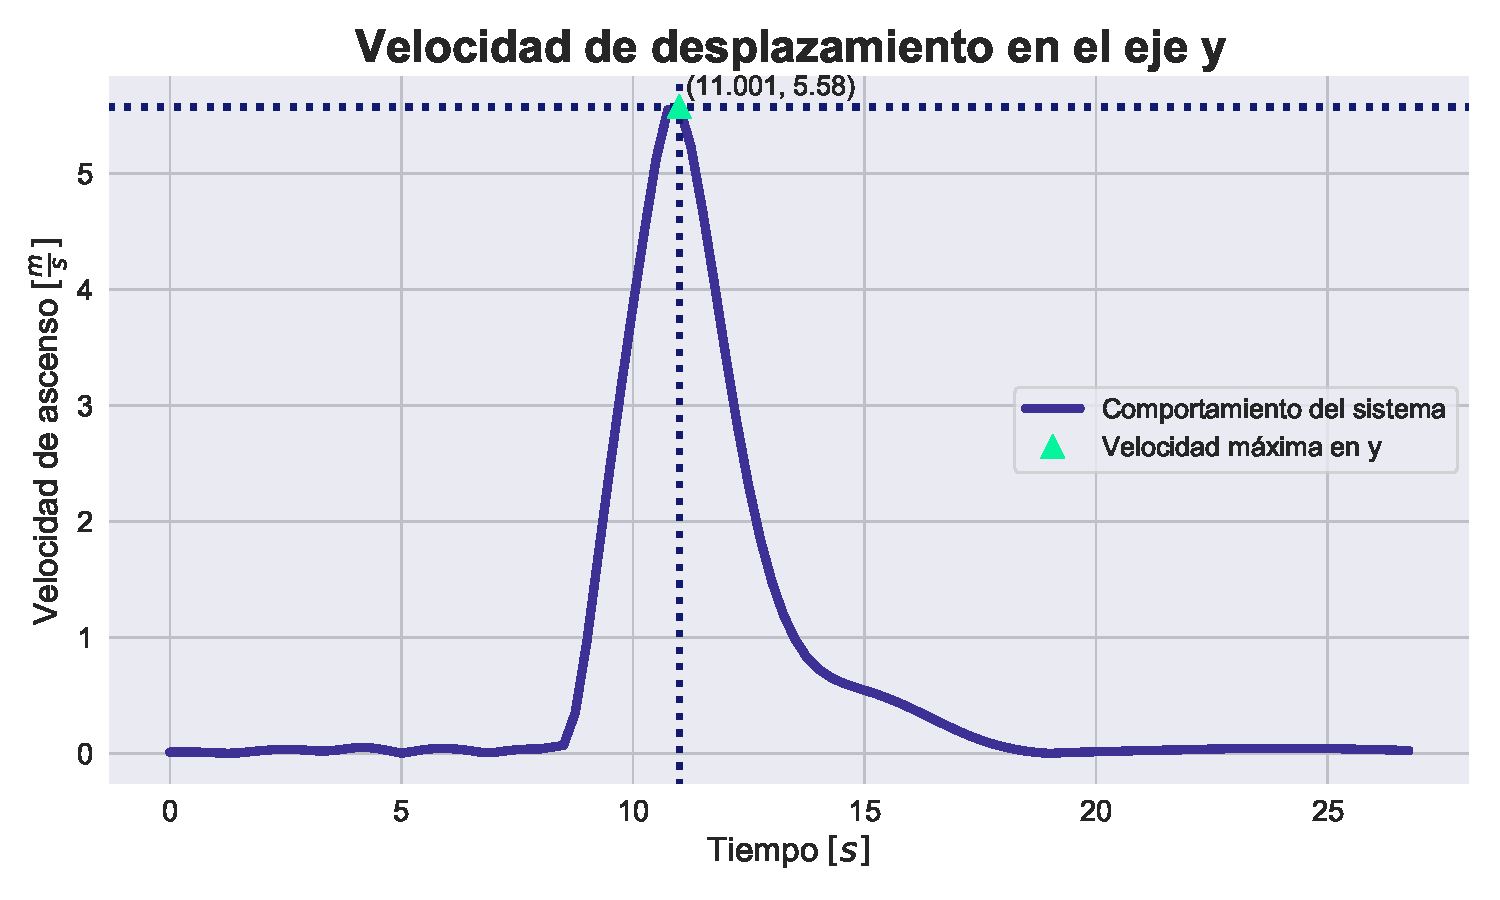
\includegraphics[width=0.48\textwidth]{pymav_movementvy.pdf}}}\\
    \subfloat[Eje Z]{\label{fig:pymav_movementvz}{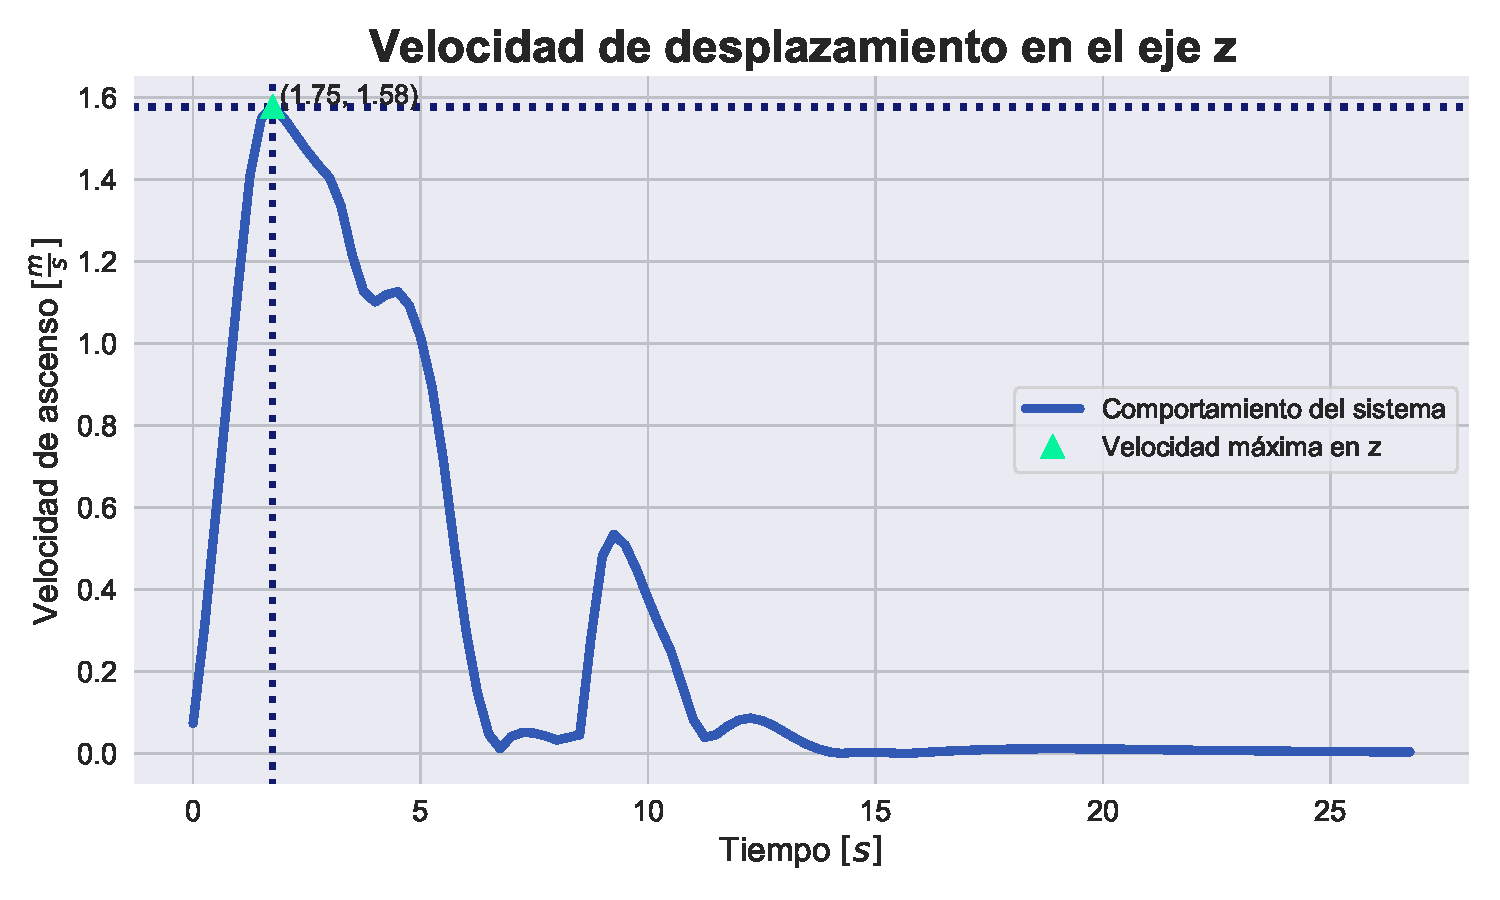
\includegraphics[width=0.48\textwidth]{pymav_movementvz.pdf}}}\hfill

    \caption{Comportamiento de la velocidad lineal de vuelo en los tres ejes}
    \label{fig:pymav_movementv}
\end{figure}

Por último con respecto a esta prueba, la figura \ref{fig:pymav_pathfollowing} presenta una proyección en 3D del la trayectoria de vuelo ejecutada por el dron. Esta gráfica presenta de manera más visual la ruta observada durante la ejecución de la simulación y es posible observar los 3 instantes más significativos de esta prueba. Primero, el dron inicia con una altura de 10 m; después se le comanda el primer waypoint [35,0,3], lo que corresponde al descenso pronunciado observado en la gráfica; cuando el dron llega a su primera referencia, se le comanda el segundo waypoint [35,17,2], donde se observa otro descenso, menos pronunciado y un movimiento a lo largo del eje \textit{y}.

\begin{figure}[ht]
    \centering
    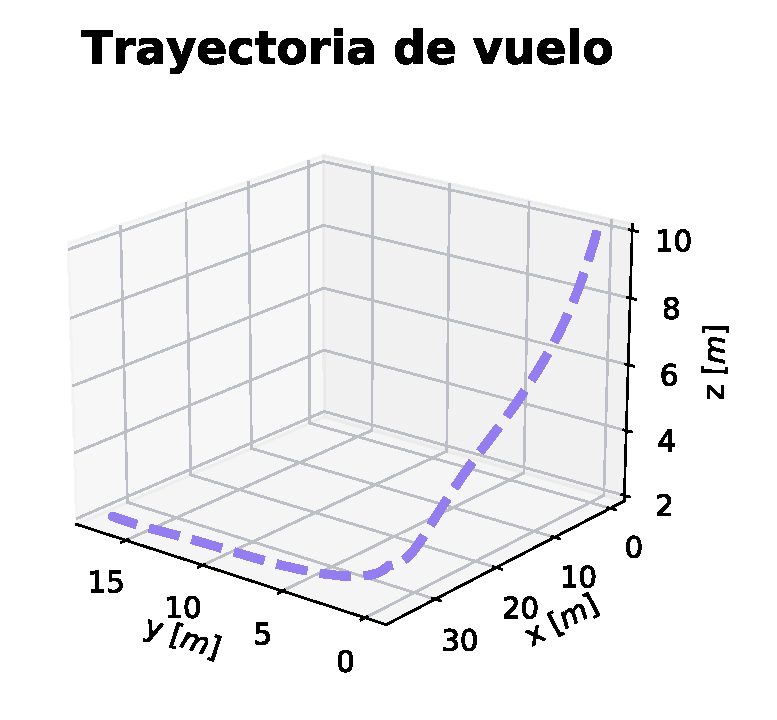
\includegraphics[width=0.45\textwidth]{pymav_pathfollowing.pdf}
    \caption{Gráfica en 3D de la trayectoria seguida por el dron.}
    \label{fig:pymav_pathfollowing}
\end{figure}

\section{Misión de vuelo}

Con la etapa anterior se culminaron las pruebas por módulos; en esta subsección se describe el proceso realizado para integrar todas las etapas descritas hasta el momento.

Debido a que se trabajó con un paradigma de módulos, en donde cada etapa descrita corresponde a un módulo y/o funcionalidad especifica, la unificación de todo lo anteriormente descrito resultó ser un proceso bastante lineal y práctico, en la mayor parte de las etapas se utilizó el mismo código desarrollado para su respectivo script; Por otro lado, en esta etapa se buscó implementar de forma completa la misión de vuelo para el dron, de tal manera que fuera capaz de cruzar a través de las 4 compuertas que componen el circuito de vuelo, por lo tanto, la misión de vuelo cuenta con 4 waypoints, los cuales se muestran en la tabla \ref{tab:waypoints_mission}.

\begin{table}[ht]
    \centering
    \begin{tabular}{ccc}
        \hline
        x & y & z\\
        \hline
        \hline
        35 & 0 & 3\\
        35 & 17 & 2\\
        0 & 17 & 3\\
        0 & 0 & 3\\
        \hline
        \hline
    \end{tabular}
    \caption{Waypoints utilizados en la misión de vuelo}
    \label{tab:waypoints_mission}
\end{table}


Dicho lo anterior, a manera de recapitulación, se describen los módulos en el orden en el que fueron implementados en el script de esta subsección:

\begin{enumerate}
    \item Establecimiento de comunicación entre Pymavlink y ArduPilot
    \item Cambio de modo de vuelo de stabilize a guided
    \item Armado de motores
    \item Envío de orden de despegue
    \item Envío de comandos de vuelo para seguimiento de waypoints
\end{enumerate}

Adicionalmente, el script de misión de vuelo busca eliminar la necesidad de que el usuario tenga que introducir comando de vuelo de forma manual en la terminal de ArduPilot; es decir, solo es necesario ejecutar el script y el dron será capaz de ejecutar todas las etapas descritas.

Ahora bien, la figura \ref{fig:pymav_mission} muestra el comportamiento observado en simulación tras haber ejecutado el script de la misión de vuelo, de tal manera que en la figura \ref{fig:pymav_mission1} se observa como el dron es capaz de cruzar por el centro de la primera compuerta; la figura \ref{fig:pymav_mission2} presenta el cruce por la segunda compuerta; la figura \ref{fig:pymav_mission3} corresponde al waypoint para la tercera compuerta y por último en la figura \ref{fig:pymav_mission4} se observa el estado final del dron tras haber atravesado la cuarta compuerta. Entonces, a partir de la figura \ref{fig:pymav_mission} es posible apreciar, a simple vista, como el dron logró completar el circuito de vuelo de forma exitosa.  

\begin{figure}[ht]
    \centering
    \subfloat[]{\label{fig:pymav_mission1}{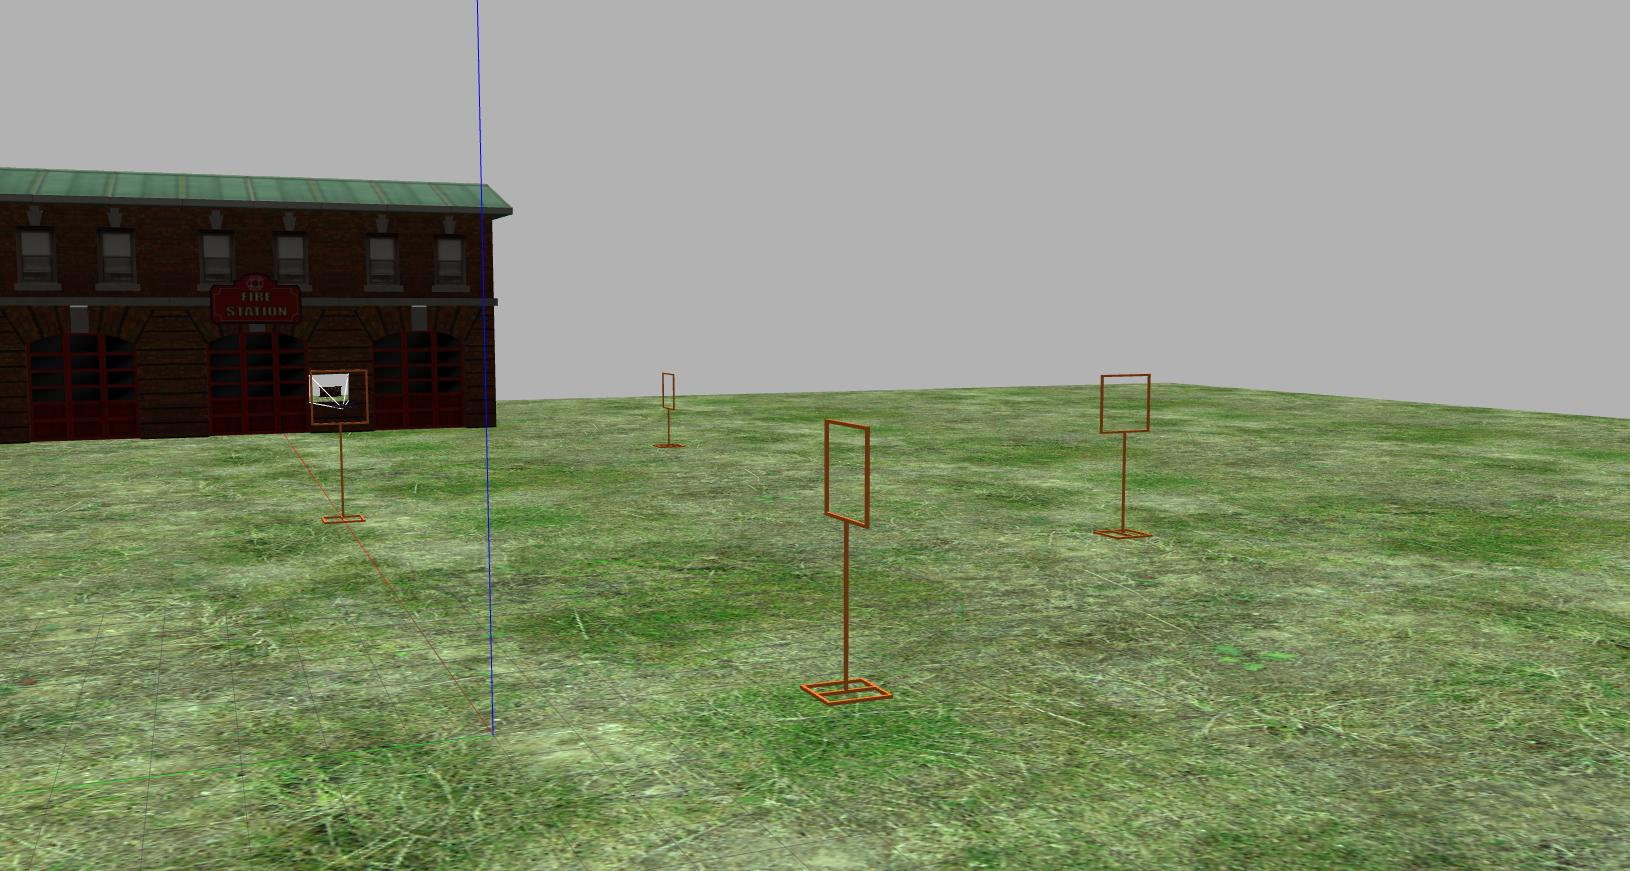
\includegraphics[width=0.48\textwidth]{pymav_mission1.jpg}}}\hfill
    \subfloat[]{\label{fig:pymav_mission2}{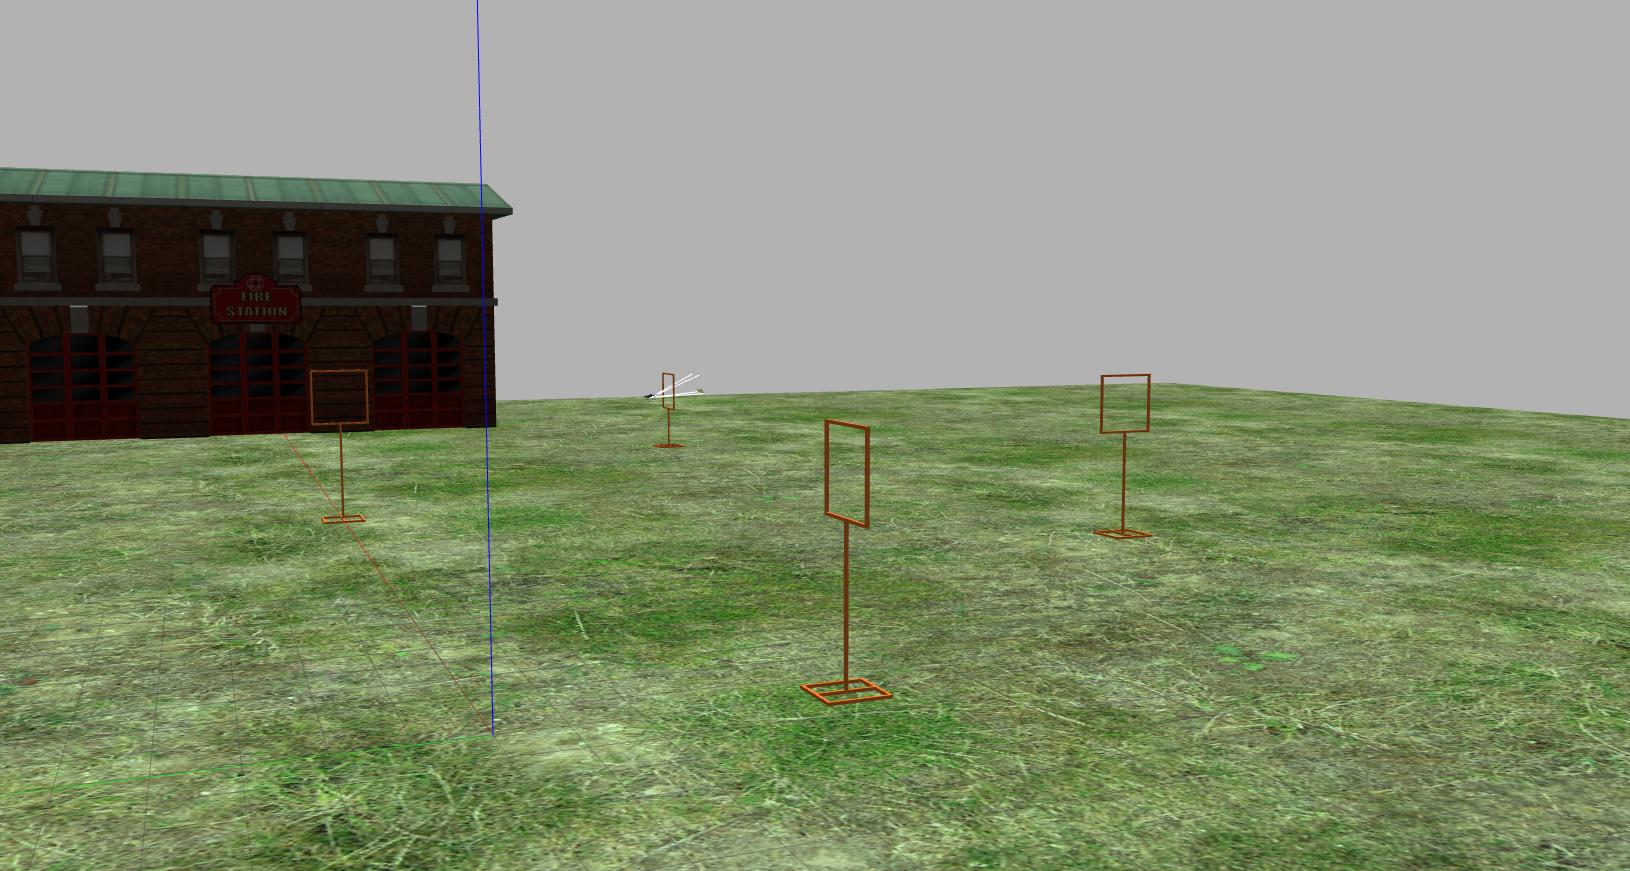
\includegraphics[width=0.48\textwidth]{pymav_mission2.jpg}}}\\
    \subfloat[]{\label{fig:pymav_mission3}{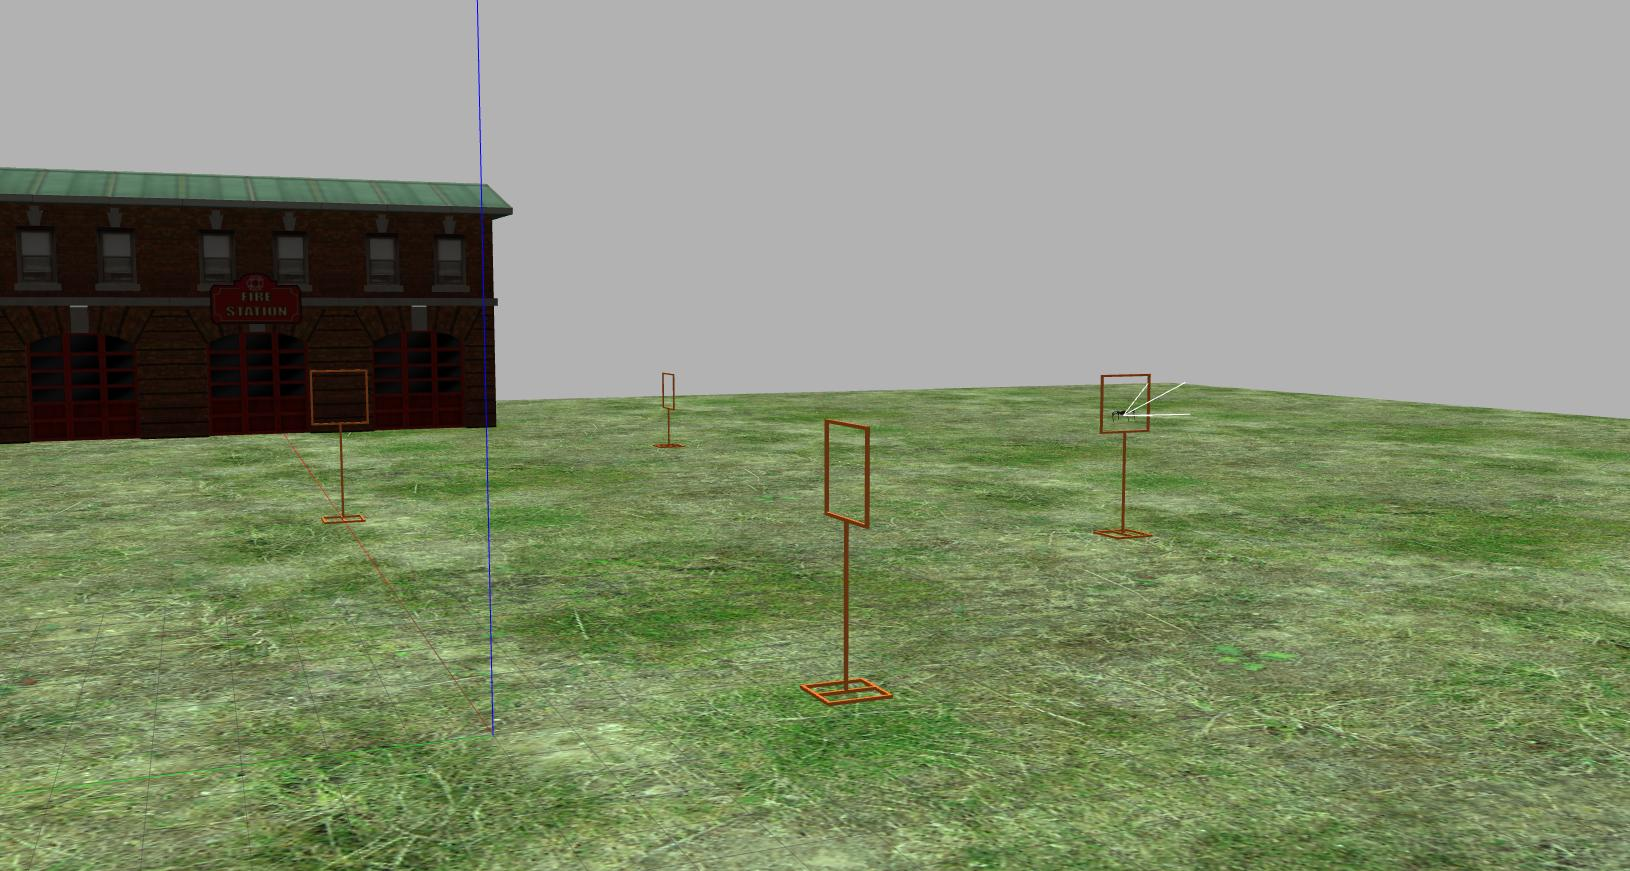
\includegraphics[width=0.48\textwidth]{pymav_mission3.jpg}}}\hfill
    \subfloat[]{\label{fig:pymav_mission4}{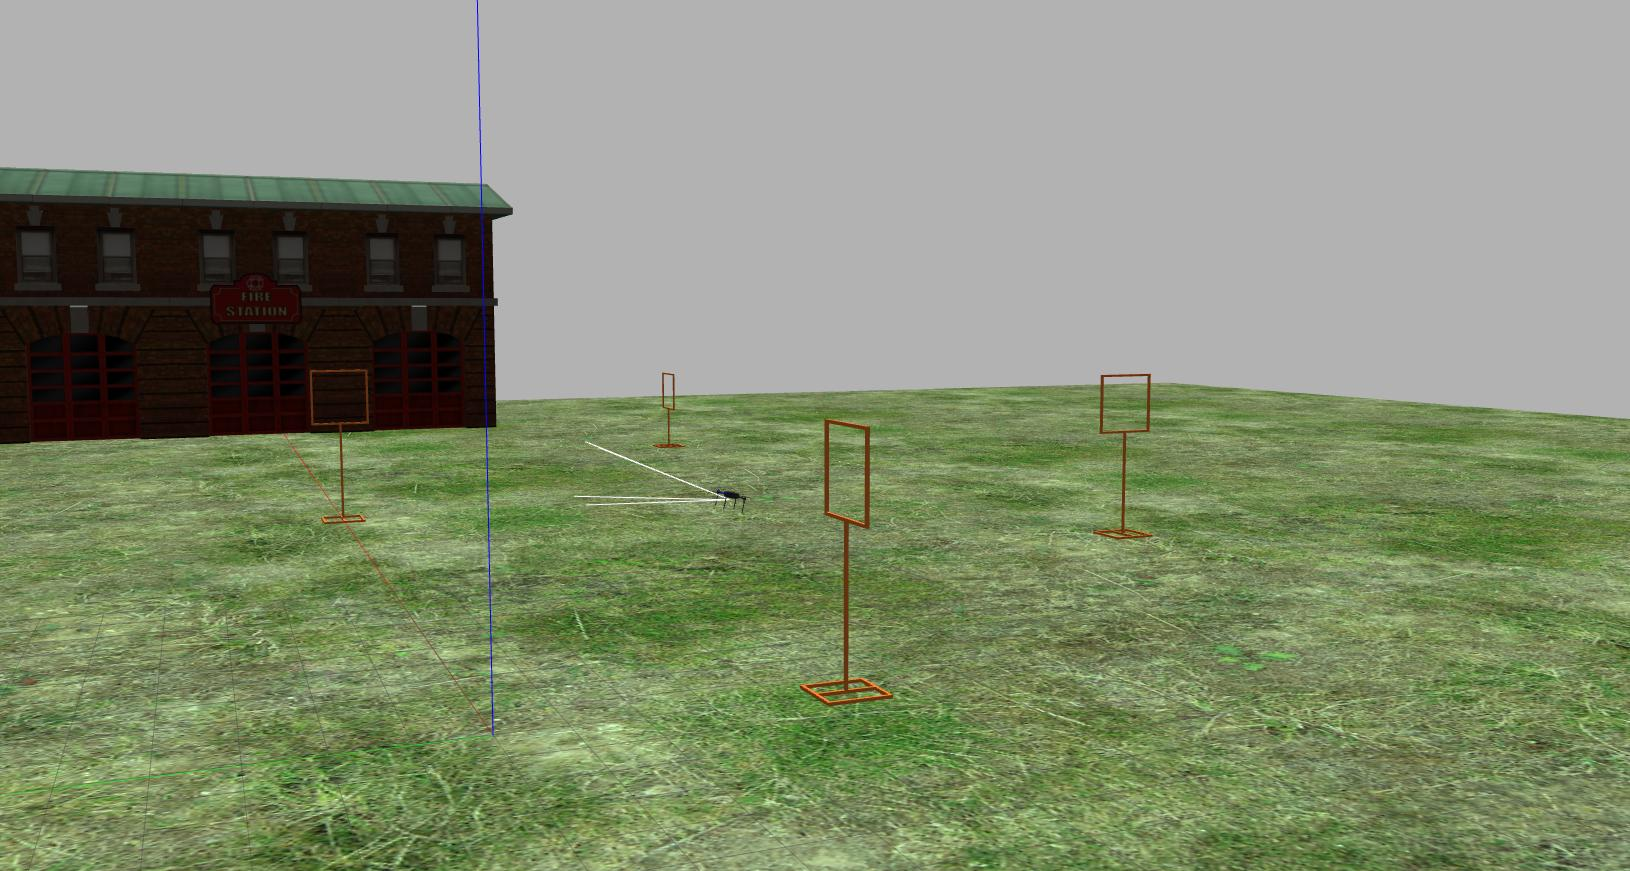
\includegraphics[width=0.48\textwidth]{pymav_mission4.jpg}}}\hfill

    \caption{Seguimiento de misión de vuelo completa}
    \label{fig:pymav_mission}
\end{figure}

De forma similar a la subsección correspondiente al seguimiento de trayectoria, la figura \ref{fig:pymav_missionxy} presenta la ruta de vuelo realizada por el dron. Se vuelve a destacar que, contraintuitivamente, el desplazamiento entre los ejes se encuentra acomodado de tal manera que correspondan a la perspectiva con la que se observó el vuelo del dron; es decir, como si se estuviera viendo el desplazamiento del dron como se observa en la figura \ref{fig:pymav_mission}. Además, la figura \ref{fig:pymav_missionxy} cuenta con la ubicación de las cuatro compuertas del circuito de vuelo, así como el sentido de vuelo que siguió el dron durante su recorrido. A partir de esto, se logra apreciar que los waypoints fueron definidos de tal manera que el dron describiera una trayectoria rectangular uniforme, por lo tanto, la trayectoria recorrida por cada waypoint corresponde a cada una de las artistas del rectángulo y la transición entre cada uno está representado por los vértices de este. 

Por otro lado, cabe mencionar que MAVLink acepta misiones de vuelo de forma nativa, en donde solo es necesario cargar un archivo de texto en donde se defina la serie de waypoints que se desean seguir, por medio de coordenadas según el marco de referencia; sin embargo, al tiempo de desarrollo de este trabajo, no se encontró ningún comando de vuelo aceptado por PymavLink que permitiera cargar de forma sencilla una misión de vuelo, por lo que, la trayectoria de vuelo implementada se realizó a partir de una función desarrollada desde cero, en donde los waypoints son enviados de forma explícita y de uno en uno, debido a esto fue necesario implementar la solución mencionada en la subsección anterior, en donde por medio de un mensaje es posible conocer la distancia restante para que el dron complete la trayectoria de cada waypoint.

\begin{figure}[ht]
    \centering
    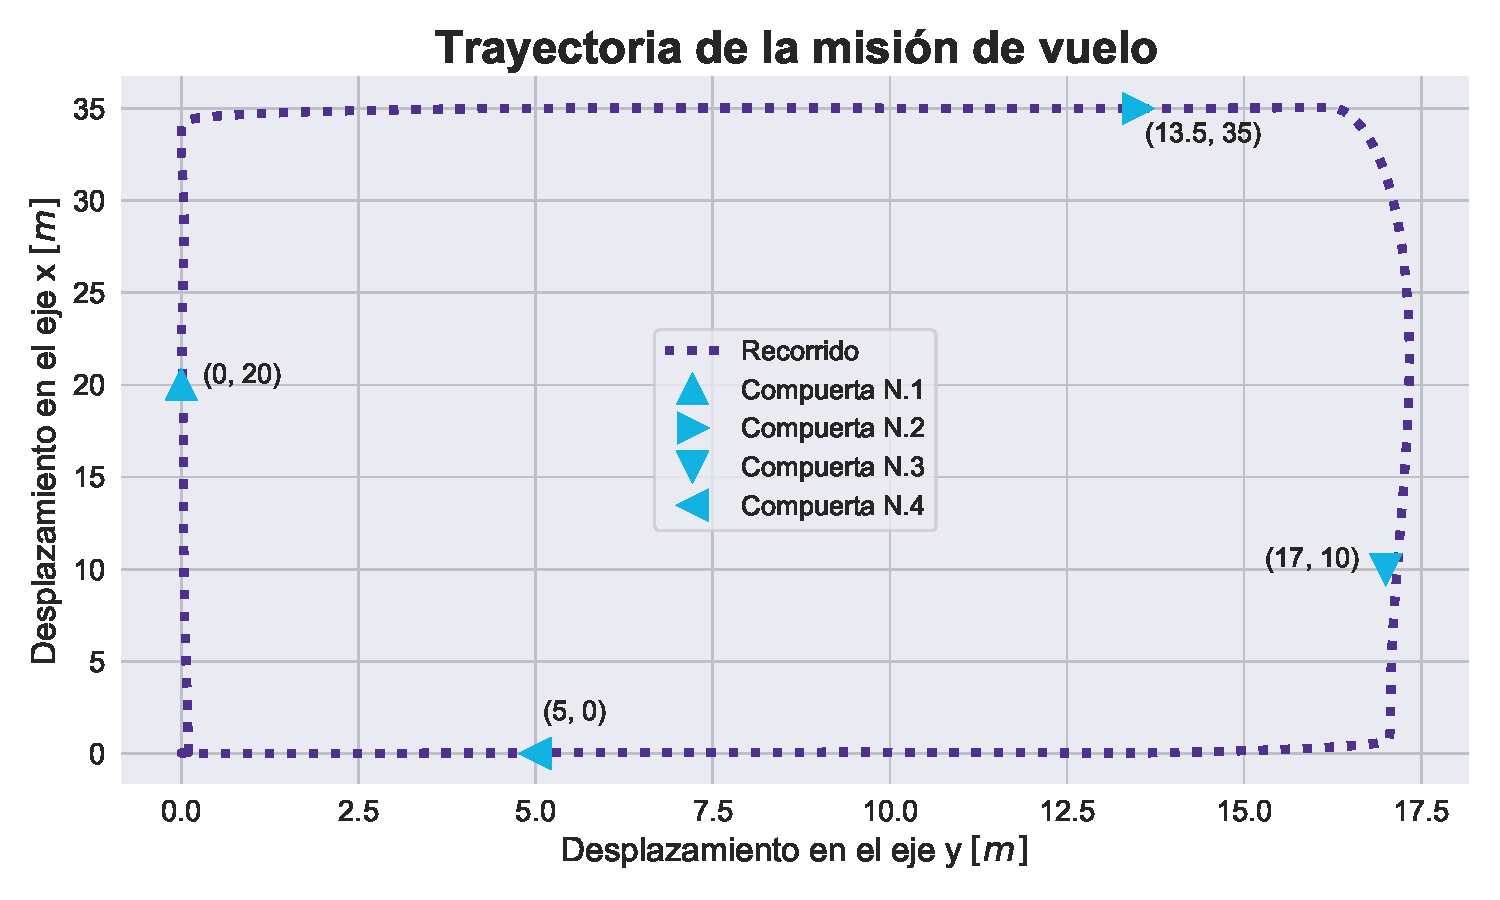
\includegraphics[width=0.75\textwidth]{pymav_missionxy.pdf}
    \caption{Recorrido realizado por el dron}
    \label{fig:pymav_missionxy}
\end{figure}

Siguiendo con los resultados obtenidos en esta subsección, la figura \ref{fig:pymav_missiond} muestra el desplazamiento lineal capturado durante el vuelo del dron. Es posible observar un comportamiento bastante peculiar en todos los ejes, por un lado en la figura \ref{fig:pymav_missionx} se puede apreciar como para el primer waypoint el desplazamiento en el eje \textit{x} incrementa de forma gradual hasta llegar a 35 m, en aproximadamente 10 segundos, después, ocurre la transición para el segundo waypoint, sin embargo la posición en el eje \textit{x} se mantiene intacta, por eso el dron permanece en 35, hasta el segundo 16, en donde ocurre la transición al tercer waypoint y es necesario disminuir el desplazamiento hasta llegar a 0 m en el eje \textit{x}, en donde el dron se mantiene hasta finalizar su recorrido. Por otro lado, en la figura \ref{fig:pymav_missiony} se aprecia un comportamiento en el eje \textit{y} de cierta forma complementario al del eje \textit{x}, en los primeros 10 segundos del recorrido, el dron no presenta ningún desplazamiento en \textit{y} por lo que su posición con respecto a este eje se mantiene en 0, posteriormente, ocurre la transición al segundo waypoint y es cuando ocurre el primer desplazamiento en \textit{y}, de tal forma que el dron avanza 17 m, después, en el segundo 25, se da la transición al tercer waypoint y la posición en \textit{y} comienza a decrementar, de tal forma que para el segundo 30 el dron ya se encuentra en el origen del circuito de vuelo. De manera similar, a partir de la figura \ref{fig:pymav_missionz} es posible intuir el comportamiento de la altura del dron durante su vuelo, el cual resulta ser más sencillo que los dos anteriores pues en este caso, la altitud solamente osciló entre dos valores 3 y 2 m, donde a los 10 segundos de vuelo ocurre un descenso a los 2 m de altura, pues ocurre la transición al segundo waypoint y la compuerta correspondiente  a este waypoinzt es de menor tamaño, por lo que es necesario que el dron descienda y luego vuelva a ascender a los 3 m cuando ocurre la siguiente transición de waypoints.

\begin{figure}[ht]
    \centering
    \subfloat[Eje X]{\label{fig:pymav_missionx}{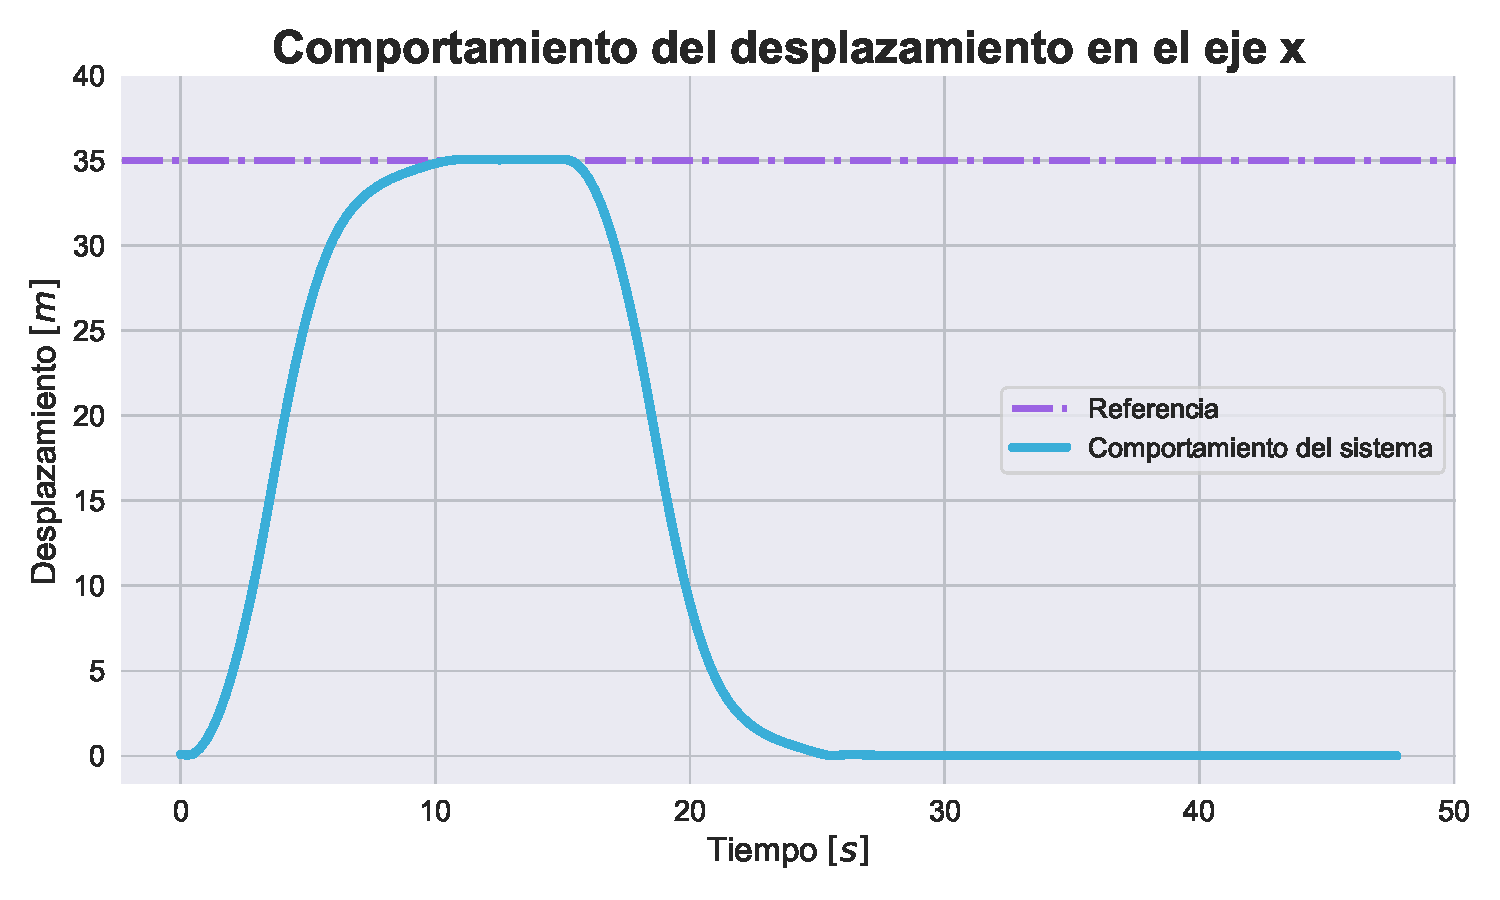
\includegraphics[width=0.48\textwidth]{pymav_missionx.pdf}}}\hfill
    \subfloat[Eje Y]{\label{fig:pymav_missiony}{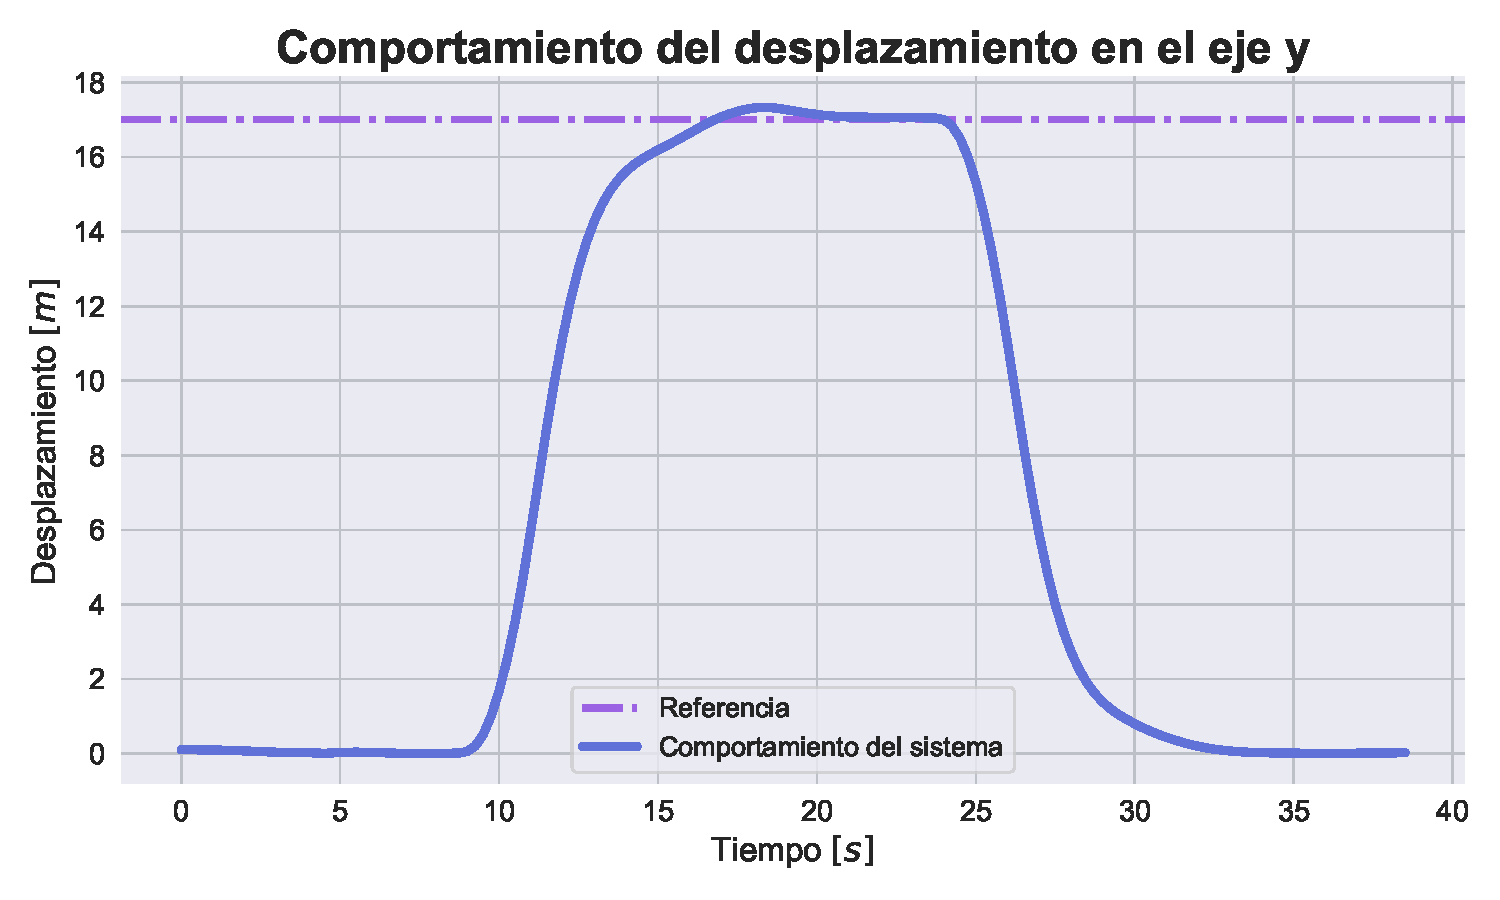
\includegraphics[width=0.48\textwidth]{pymav_missiony.pdf}}}\\
    \subfloat[Eje Z]{\label{fig:pymav_missionz}{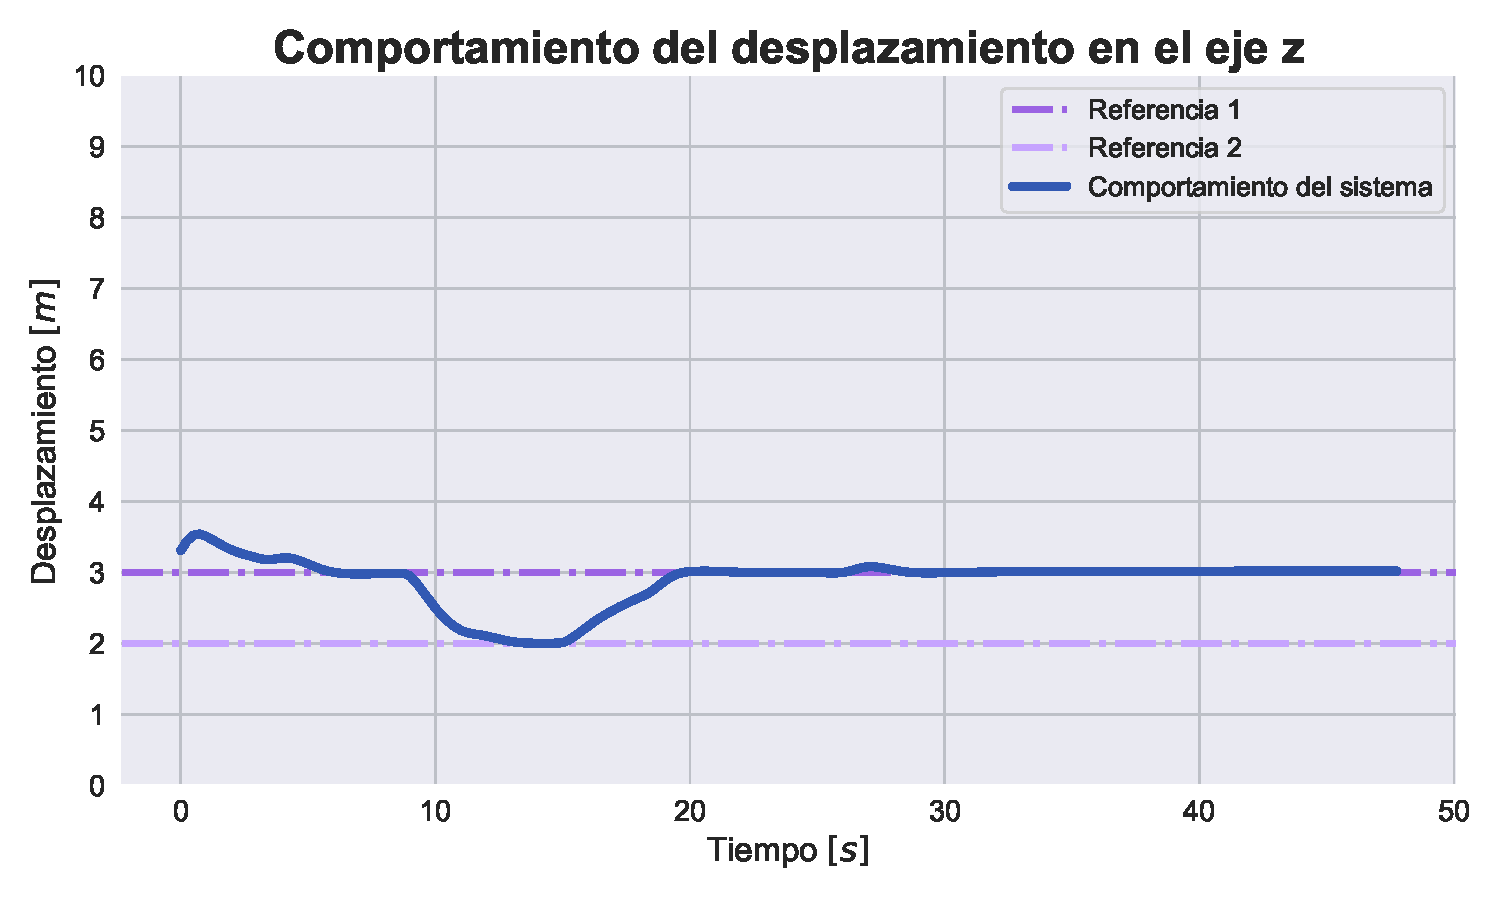
\includegraphics[width=0.48\textwidth]{pymav_missionz.pdf}}}\hfill

    \caption{Gráficas de desplazamiento para los tres ejes}
    \label{fig:pymav_missiond}
\end{figure}

 Así mismo, la figura \ref{fig:pymav_missionv} presenta el comportamiento de la velocidad lineal en los tres ejes de desplazamiento. La gráfica de la figura \ref{fig:pymav_missionvx} presenta el comportamiento en el eje \textit{x}, mientras que la figura \ref{fig:pymav_missionvy} hace lo respectivo con el eje \textit{y}; como se observa, ambas gráficas presentan comportamientos bastantes similares. El primer waypoint 35,0,3 involucra un desplazamiento positivo en el eje \textit{x}, sin desplazarse en el eje \textit{y}, por lo que en los primeros 10 segundos de la simulación se observa el máximo en $v_x$ de 8.42 $\frac{m}{s}$, mientras que $v_y$ permanence en 0; el decremento de $v_x$ se debe a que el dron comienza a detenerse conforme se acerca a la referencia de posición, y poco antes del segundo 10 se observa un incremento en $v_y$, debido a la transición al segundo waypoint 35,17,2, donde $v_y$ alcanza su máximo de 5.53 $\frac{m}{s}$ en el segundo 11.25 para después disminuir su velocidad.
 
 Luego, se observa una pendiente negativa en $v_x$ pues el tercer waypoint [0,17,3] implica un retroceso en el desplazamiento en \textit{x}, de tal forma que después del segundo 18.5 también se observa una reducción en la magnitud de $v_x$ hasta llegar a cero. Este comportamiento también se observa para el cuarto waypoint [0,0,0] en donde $v_y$ presenta la pendiente negativa y posteriormente un detenimiento completo.

 Por último, en la figura \ref{fig:pymav_missionvz} es posible observar el comportamiento de $v_z$. Se aprecia que al inicio de la gráfica se presenta el máximo de velocidad (0.67 $\frac{m}{s}$), esto se debe a que la adquisición de datos comenzó justo después de que la etapa de despegue hubiera concluido, por lo que el dron ya contaba con cierta velocidad, después de eso, se observan decrementos graduales en $v_z$ con el fin de detener su movimiento, por la llegada a la altura de referencia; sin embargo, en el segundo 10 ocurre el comando del segundo waypoint, el cual cambia la referencia a 2 m, por lo que el dron tuvo que descender para alcanzar esa altura, y posteriormente, el tercer waypoint provoco que el dron volviera a ascender, debido a esto se observa picos positivos en el segundo 15 aproximadamente. 

\begin{figure}[ht]
    \centering
    \subfloat[Eje X]{\label{fig:pymav_missionvx}{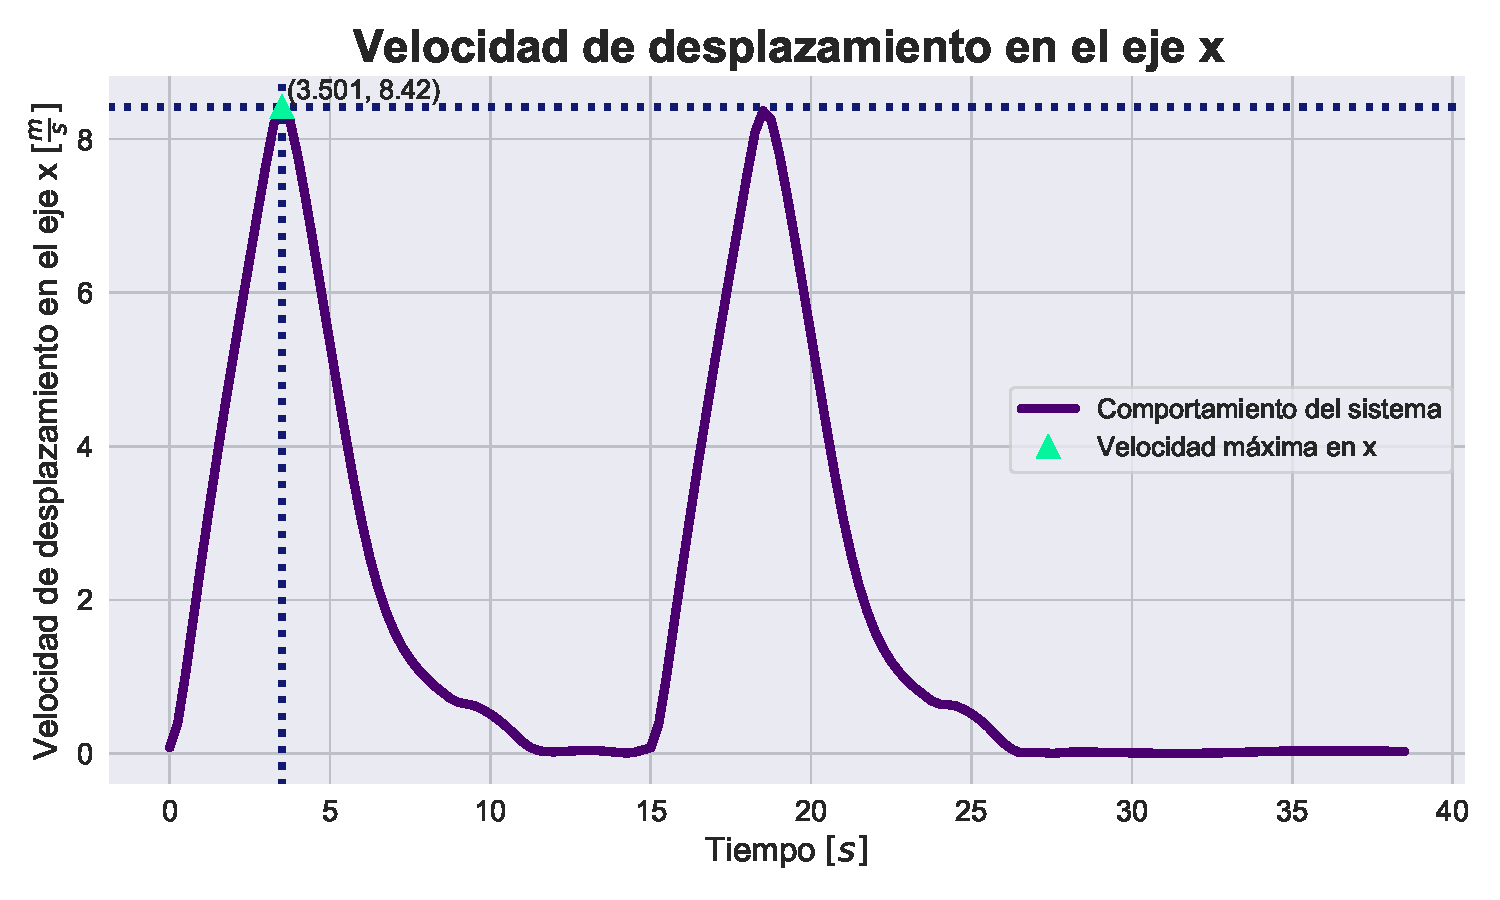
\includegraphics[width=0.48\textwidth]{pymav_missionvx.pdf}}}\hfill
    \subfloat[Eje Y]{\label{fig:pymav_missionvy}{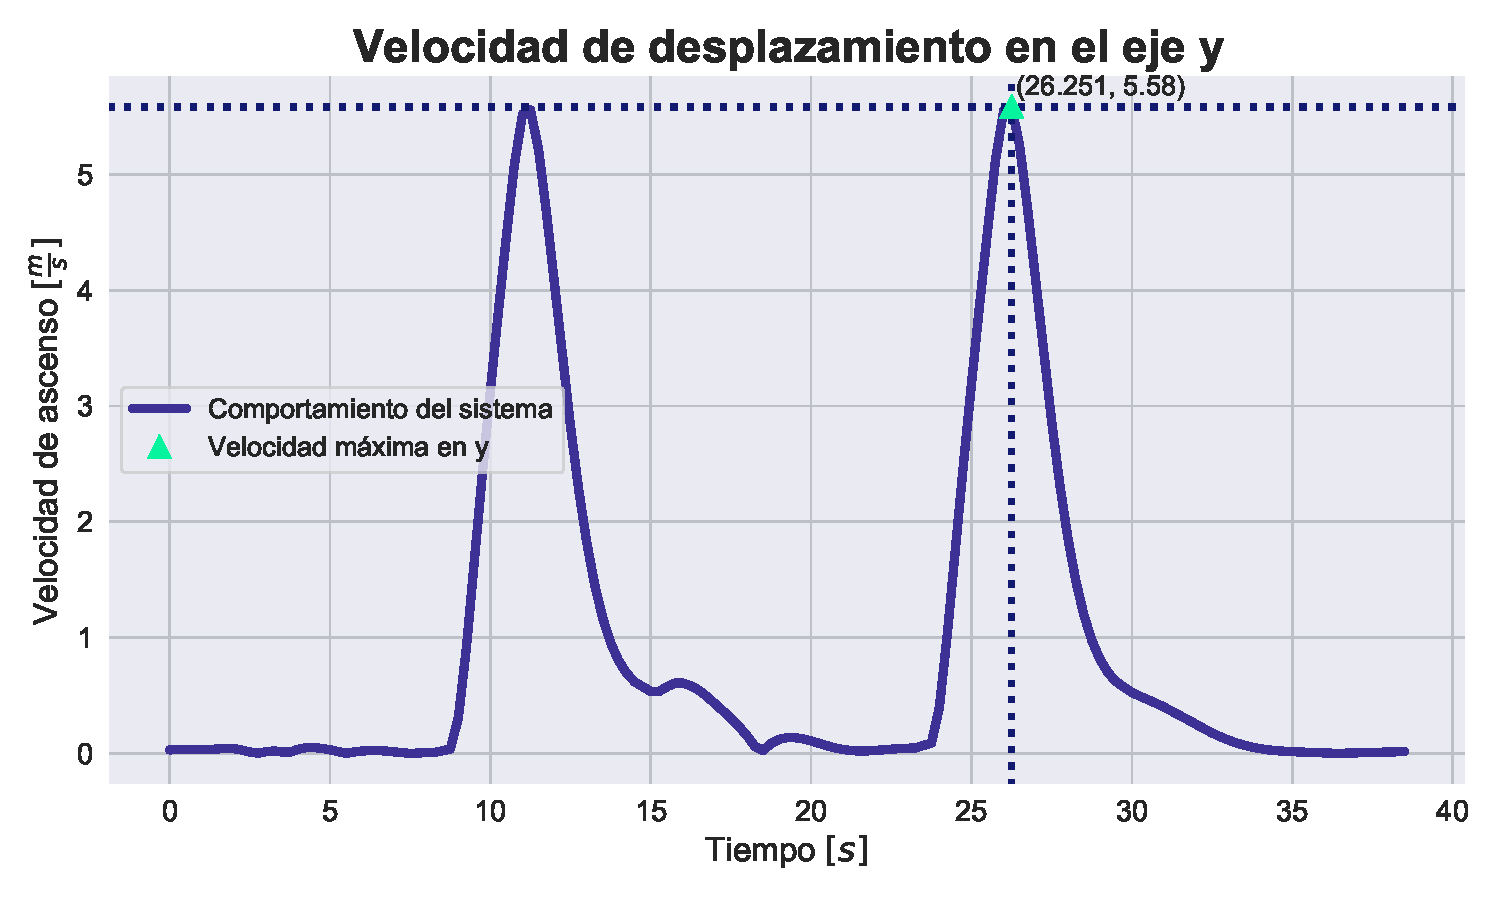
\includegraphics[width=0.48\textwidth]{pymav_missionvy.pdf}}}\\
    \subfloat[Eje Z]{\label{fig:pymav_missionvz}{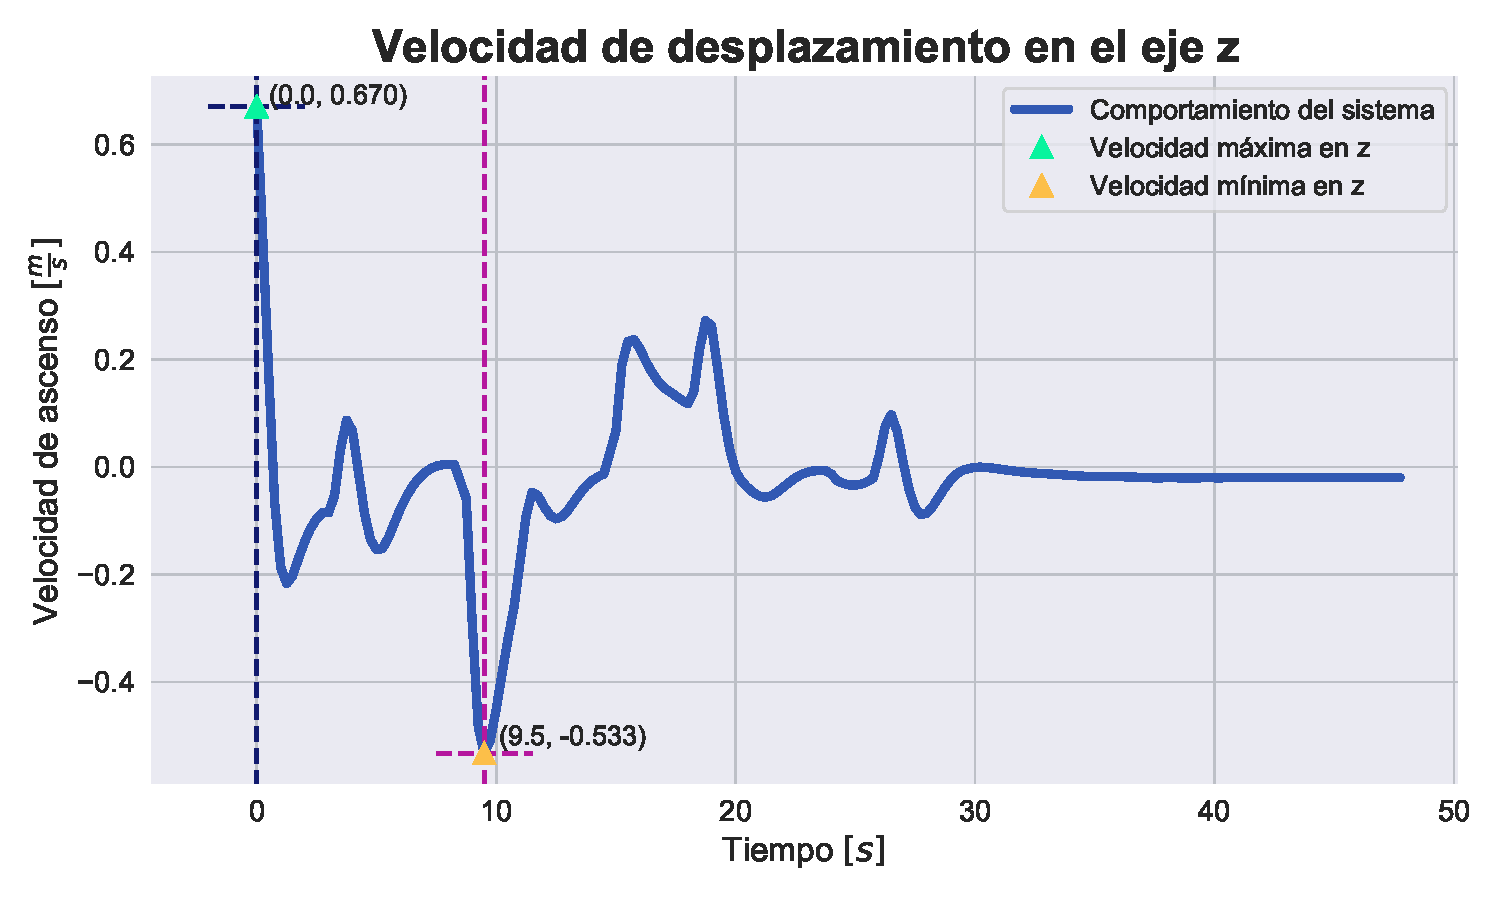
\includegraphics[width=0.48\textwidth]{pymav_missionvz.pdf}}}\hfill

    \caption{Comportamiento de la velocidad lineal de vuelo en los tres ejes}
    \label{fig:pymav_missionv}
\end{figure}




\section{Aterrizaje (extra)}

Por último, con respecto al algoritmo de seguimiento de trayectoria, esta subsección se maneja como extra debido a que en la implementación final, el dron no realiza la secuencia de aterrizaje, pues se decidió que completara el circuito de forma indefinida. Sin embargo, se consideró que es importante mencionar que durante las pruebas realizadas sí se implementó una lógica que permitiera aterrizar el dron una vez que completo el circuito de vuelo. 

Se consideraron dos posibles implementaciones para el aterrizaje, la primera, utilizar 2 waypoints más para guiar al dron hacía el origen y, por otro lado, el uso del modo de vuelo integrado en el piloto automático. La segunda opción resultó ser más factible, pues al utilizar waypoints para el descenso del dron, este lo hace de forma brusca y al entrar en contacto con el suelo se observa un rebote derivado de la velocidad de descenso.

Entonces, para implementar el modo de vuelo de aterrizaje, se realizó el mismo proceso implementado en la subsección de la secuencia de despegue, la diferencia se encuentra en que ahora el modo de vuelo especificado es \textit{LAND}, y por supuesto, en este caso no se requiere enviar el comando de vuelo para el despegue.
